% longtable v4.24 (10/2025) báo "Infinite glue shrinkage" ở mọi chỗ bảng ngắt trang; dùng bản v4.13 kèm sẵn.
\makeatletter\declare@file@substitution{longtable.sty}{longtable-2020-01-07.sty}\makeatother
\PassOptionsToPackage{table}{xcolor}
\documentclass[twoside,final]{hcmut-report}
\usepackage{pdflscape}
\usepackage{array}
\usepackage{longtable}
\usepackage{xcolor}

\setlength{\LTleft}{0pt}
\setlength{\LTright}{0pt}
\setlength{\emergencystretch}{3em}

\definecolor{codebg}{gray}{0.96}
\definecolor{codecomment}{rgb}{0.25,0.45,0.25}
\definecolor{codekeyword}{rgb}{0.10,0.20,0.55}
\lstdefinestyle{cpp}{
  language=C++, basicstyle=\ttfamily\scriptsize, keywordstyle=\color{codekeyword}\bfseries,
  commentstyle=\color{codecomment}\itshape, backgroundcolor=\color{codebg}, frame=single,
  rulecolor=\color{gray!60}, numbers=left, numberstyle=\tiny\color{gray}, numbersep=6pt,
  breaklines=true, breakatwhitespace=true, columns=fullflexible, keepspaces=true,
  showstringspaces=false, tabsize=4, captionpos=t, xleftmargin=1.5em, framexleftmargin=1.5em,
  morekeywords={noexcept,constexpr,nullptr,alignas,template,typename,using}
}
\lstset{style=cpp}
\renewcommand{\lstlistingname}{Listing}
\renewcommand{\lstlistlistingname}{List of Listings}
\newcommand{\src}{../..}

\newcommand{\RunID}{run-laptop-02}
\newcommand{\SourceSHA}{38a67327a7a796b185cbda8610e235bfac08c2ab067e2ebacf906cfeffe9a8b2}
\newcommand{\NumConfigs}{711}
\newcommand{\NumSamples}{6399}
\newcommand{\NumFailedMeasured}{0}
\newcommand{\NumFailedWarmups}{1}
\newcommand{\Warmups}{2}
\newcommand{\Reps}{7}
\newcommand{\TimeoutS}{60}
\newcommand{\OrderSeed}{20261016}
\newcommand{\CPUModel}{13th Gen Intel\textsuperscript{\textregistered} Core\texttrademark i7-13620H}
\newcommand{\PhysCores}{10}
\newcommand{\LogicalCPUs}{16}
\newcommand{\MemGiB}{15.7}
\newcommand{\OSName}{Windows-11-10.0.26200-SP0}
\newcommand{\Compiler}{g++.exe (Rev3, Built by MSYS2 project) 13.2.0}
\newcommand{\CMakeVersion}{cmake version 4.2.1}
\newcommand{\ReleaseFlags}{-O3 -DNDEBUG}
\newcommand{\PowerScheme}{Legion Balance Mode}
\newcommand{\ACState}{AC power}
\newcommand{\SpinHint}{x86\_pause}
\newcommand{\ThreadList}{1, 2, 3, 4, 6, 8, 10, 12, 14}
\newcommand{\MeasureDate}{2026-10-24}


\coursename{Parallel Computing (CO5133)}
\reporttype{Assignment 1 Report}
\title{Shared-Memory Synchronization: Spinlocks, a Sense-Reversing Barrier and Concurrent Counters}
\advisor{Dr. Diep Thanh Dang}
\stuname{Nguyễn Hữu Phúc}
\newcommand{\stuid}{2352938}

% Same cover as hcmut-report.cls, but one advisor, no group row, and the student ID on its own row.
\makeatletter
\renewcommand{\coverpage}{
  \pagestyle{empty}
  \vspace*{-3\baselineskip}
  \begin{center}
    \MakeUppercase{\@upperuniname}

    \MakeUppercase{\@uniname}

    \MakeUppercase{\@deptname}
    \vfill
    
\includegraphics[scale=0.4]{graphics/hcmut.png}
    \vfill
    \bfseries
    \begin{tabular}{c}
      \Large\@coursename                                 \\
      {}                                                 \\
      \midrule                                           \\
      {}                                                 \\
      \Large\@reporttype                                 \\
      {}                                                 \\
      \Huge\parbox[c]{0.8\linewidth}{\centering \@title} \\
      {}                                                 \\
      \bottomrule
    \end{tabular}
    \vfill
    \mdseries
    \begin{tabular}{rl}
      Advisor: & \@advisor \\
      Student: & \@stuname \\
      Student ID: & \stuid \\
    \end{tabular}
    \vfill
    \MakeUppercase{\@reportplace, \@reporttime}
  \end{center}
  \clearpage
  \pagestyle{fancy}
}
\makeatother

\begin{document}

\coverpage%

\section*{Abstract}
\addcontentsline{toc}{section}{Abstract}

This report presents the implementation, correctness testing and performance study of three classes of shared-memory synchronization required by Assignment~1: the TAS, TTAS and MCS spinlocks, a reusable Sense-Reversing Barrier, and concurrent counters built on mutual exclusion, compare-and-swap (CAS) and fetch-and-add (FAA). All are written in C++20 with explicit memory orders that follow the acquire/release discipline of the course, and are compared with \texttt{std::mutex} and \texttt{std::barrier}. Exponential backoff is evaluated as a variant of TTAS and of the CAS counter.

Correctness is tested by property-based multi-threaded tests, directed tests that force rare interleavings such as the MCS enqueue gap, sequentially consistent reference variants, stress runs, and AddressSanitizer, UndefinedBehaviorSanitizer and ThreadSanitizer builds; every check passes. Performance is measured on a 16-thread hybrid laptop CPU with \NumSamples{} process-level samples. Spinlocks approach the Amdahl bound at low thread counts while \texttt{std::mutex} is slower than a single thread whenever half of the work is outside the lock. MCS collapses once spinning threads occupy every logical CPU, because a preempted successor blocks its FIFO queue. The spinning barrier outperforms \texttt{std::barrier} by about two orders of magnitude up to 12 threads, and no counter becomes faster than a single thread.

\textbf{Keywords:} spinlock, MCS lock, sense-reversing barrier, compare-and-swap, fetch-and-add, C++ memory model, exponential backoff, scalability.

\newpage
\tableofcontents
\newpage
\section*{List of Abbreviations}
\addcontentsline{toc}{section}{List of Abbreviations}

{\small
\begin{longtable}{|>{\raggedright\arraybackslash}p{\dimexpr 0.25\textwidth-2\tabcolsep-\arrayrulewidth\relax}|>{\raggedright\arraybackslash}p{\dimexpr 0.745\textwidth-2\tabcolsep-\arrayrulewidth\relax}|}
\hline
\textbf{Abbreviation} & \textbf{Expansion} \\ \hline
\endfirsthead
\hline
\textbf{Abbreviation} & \textbf{Expansion} \\ \hline
\endhead
ASan & AddressSanitizer \\ \hline
CAS & Compare-and-swap (\texttt{compare\_exchange} in C++) \\ \hline
CS & Critical section \\ \hline
E-core / P-core & Efficiency core / performance core of a hybrid Intel CPU \\ \hline
FAA & Fetch-and-add (\texttt{fetch\_add} in C++) \\ \hline
FIFO & First in, first out \\ \hline
HT & Hyper-Threading (two hardware threads per core) \\ \hline
IQR & Interquartile range (first to third quartile) \\ \hline
LTO & Link-time optimization \\ \hline
MCS & Mellor-Crummey and Scott queue lock \\ \hline
MPI & Message Passing Interface \\ \hline
RMA & Remote memory access (MPI one-sided communication) \\ \hline
RMW & Read-modify-write atomic operation \\ \hline
SC & Sequential consistency (\texttt{memory\_order\_seq\_cst}) \\ \hline
TAS & Test-and-set lock \\ \hline
TSan & ThreadSanitizer \\ \hline
TTAS & Test-and-test-and-set lock \\ \hline
UBSan & UndefinedBehaviorSanitizer \\ \hline
\end{longtable}
}

\newpage
\listoffigures
\addcontentsline{toc}{section}{List of Figures}
\listoftables
\addcontentsline{toc}{section}{List of Tables}
\lstlistoflistings
\addcontentsline{toc}{section}{List of Listings}

\newpage
\section{Introduction}\label{sec:intro}

\subsection{Assignment overview}

Assignment~1\cite{r1} asks for three shared-memory synchronization mechanisms discussed in the lecture, each to be implemented in C++, tested for correctness and studied for performance and scalability on the shared-memory platforms the student owns:

\begin{enumerate}[leftmargin=1.5em]
  \item \textbf{Mutex locks.} The TAS, TTAS and MCS spinlocks, exercised by a program in which every thread repeatedly acquires the lock, checks whether a number $N$ is prime inside the critical section, releases the lock and then performs \texttt{OUTSIDE\_WORK} further primality checks outside it. The metric is the execution time of the whole program, and the locks are to be compared with existing mutex implementations.
  \item \textbf{Barrier synchronization.} A Sense-Reversing Barrier, measured by the number of completed barrier episodes per unit time with no useful work between barriers, and compared with existing barriers.
  \item \textbf{Concurrent counters.} Counters synchronized by mutex locks, compare-and-swap and fetch-and-add, measured by execution time.
\end{enumerate}

Exponential backoff is suggested for mutex locks, barriers and counters, and a fourth part on distributed versions using MPI-3 one-sided communication is optional.

\subsection{Requirements and where they are addressed}

Table~\ref{tab:requirements} lists every requirement of the statement and the part of this report that addresses it.

{\small
\begin{longtable}{|>{\raggedright\arraybackslash}p{\dimexpr 0.07\textwidth-2\tabcolsep-\arrayrulewidth\relax}|>{\raggedright\arraybackslash}p{\dimexpr 0.48\textwidth-2\tabcolsep-\arrayrulewidth\relax}|>{\raggedright\arraybackslash}p{\dimexpr 0.445\textwidth-2\tabcolsep-\arrayrulewidth\relax}|}
\caption[Assignment requirements and where this report addresses them]{Assignment requirements\cite{r1} and where this report addresses them.}\label{tab:requirements} \\
\hline
\textbf{ID} & \textbf{Requirement} & \textbf{Addressed in} \\ \hline
\endfirsthead
\hline
\textbf{ID} & \textbf{Requirement} & \textbf{Addressed in} \\ \hline
\endhead
L1 & Implement TAS, TTAS and MCS for multi-threaded C++ programs & Sections~\ref{sec:impl-tas}--\ref{sec:impl-mcs}, Listings~\ref{lst:tas}--\ref{lst:mcs} \\ \hline
L2 & Devise an approach to testing their correctness & Section~\ref{sec:testing} \\ \hline
L3 & Test the locks in the given program: \texttt{is\_prime(N)} inside the lock, \texttt{OUTSIDE\_WORK} calls outside, \texttt{NUM\_OF\_THREADS} and \texttt{NUM\_OF\_ITERS} & Section~\ref{sec:impl-workload}, Table~\ref{tab:macro-map} \\ \hline
L4 & Performance and scalability study by execution time of the whole program while tuning the parameters & Sections~\ref{sec:method} and~\ref{sec:res-locks}--\ref{sec:res-saturation} \\ \hline
L5 & Compare with existing mutex locks & \texttt{std::mutex} in every lock experiment, Section~\ref{sec:res-stdmutex} \\ \hline
L6 & Exponential backoff for locks & TTAS with backoff, Sections~\ref{sec:impl-backoff} and~\ref{sec:res-backoff} \\ \hline
B1 & Implement the Sense-Reversing Barrier in C++ & Section~\ref{sec:impl-barrier}, Listing~\ref{lst:barrier} \\ \hline
B2 & Devise an approach to testing its correctness & Section~\ref{sec:testing} \\ \hline
B3 & Study performance and scalability by completed episodes per unit time with no useful work between barriers & Sections~\ref{sec:metrics} and~\ref{sec:res-barrier} \\ \hline
B4 & Compare with existing barriers & \texttt{std::barrier}, Section~\ref{sec:res-barrier} \\ \hline
C1 & Implement concurrent counters with mutex locks, CAS and FAA & Section~\ref{sec:impl-counters}, Listings~\ref{lst:mutex-counter}--\ref{lst:faa} \\ \hline
C2 & Devise an approach to testing their correctness & Section~\ref{sec:testing} \\ \hline
C3 & Study performance and scalability by execution time; backoff may be used & Section~\ref{sec:res-counters}; CAS with backoff \\ \hline
X1 & Run the studies on all shared-memory platforms the student owns & Section~\ref{sec:platform} \\ \hline
O1 & Distributed versions with MPI-3 one-sided communication (optional) & Not implemented; Section~\ref{sec:future} \\ \hline
S1 & Submit a ZIP with the final PDF report and all relevant C++ source code & Appendix~\ref{app:repro} \\ \hline
\end{longtable}
}

\subsection{Scope}

All three required parts are implemented, tested and measured. Two variants are added beyond the minimum: TTAS with exponential backoff and a CAS counter with exponential backoff. The barrier has no backoff variant. Each sequentially consistent (SC) variant of the custom algorithms is used only as a reference in the tests. The optional MPI-3 part is not implemented.

The study runs on one platform, the student's laptop, which is the only shared-memory machine the student owns. It is described in Section~\ref{sec:platform}.

\subsection{Report structure}

Section~\ref{sec:background} summarizes the course material the implementation relies on. Section~\ref{sec:impl} presents the implementation with its source code, and Section~\ref{sec:testing} the correctness testing approach and its results. Section~\ref{sec:method} describes the experimental method, Section~\ref{sec:results} the results, and Section~\ref{sec:conclusion} concludes. The appendices contain the complete result tables and the commands that reproduce every number in this report.

\newpage
\section{Background}\label{sec:background}

This section summarizes the course material\cite{r2} that the implementation in Section~\ref{sec:impl} is built on.

\subsection{Memory ordering and happens-before}

Cache coherence guarantees that all cores agree on the order of writes to a \emph{single} location, but it says nothing about the order in which writes to \emph{different} locations become visible. Most hardware therefore implements a relaxed memory model, and synchronizing operations must restrict reordering explicitly. The slides write such a restriction as $P\|S$: preceding accesses of kind $P$ may not move after the operation, and subsequent accesses of kind $S$ may not move before it. A lock acquire needs $\|RW$ so that the critical section cannot move above it, and a release needs $RW\|$ so that the critical section cannot move below it.

C++ expresses the same idea through the \emph{happens-before} relation. Two conflicting accesses to a non-atomic object that are not ordered by happens-before form a data race, which is undefined behavior. Between threads, happens-before is established when a release store \emph{synchronizes with} an acquire load that reads the stored value. Table~\ref{tab:orders} maps the slide notation to the C++ orders used in this work.

\begin{table}[H]
\centering
\small
\caption{Ordering restrictions in the slide notation and their C++ counterparts.}\label{tab:orders}
\begin{tabular}{|>{\raggedright\arraybackslash}p{\dimexpr 0.17\textwidth-2\tabcolsep-\arrayrulewidth\relax}|>{\raggedright\arraybackslash}p{\dimexpr 0.31\textwidth-2\tabcolsep-\arrayrulewidth\relax}|>{\raggedright\arraybackslash}p{\dimexpr 0.515\textwidth-2\tabcolsep-\arrayrulewidth\relax}|}
\hline
\textbf{Slides} & \textbf{C++ order} & \textbf{Use in this work} \\ \hline
$\|RW$ (acquire) & \texttt{memory\_order\_acquire} & Successful lock RMW, waiting loads that end a wait \\ \hline
$RW\|$ (release) & \texttt{memory\_order\_release} & Lock release, MCS handoff, barrier sense flip \\ \hline
$RW\|RW$ & \texttt{memory\_order\_acq\_rel} & MCS tail exchange, barrier arrival counter \\ \hline
none & \texttt{memory\_order\_relaxed} & Polling hints, counter values that publish no other data \\ \hline
total order & \texttt{memory\_order\_seq\_cst} & Reference variants in the tests only \\ \hline
\end{tabular}
\end{table}

Sequential consistency is stronger than acquire/release because it also imposes one total order on all SC operations. The algorithms in this assignment only need pairwise publication from one thread to the next, so acquire/release is sufficient, and SC variants serve as a cross-check in the tests.

\subsection{Atomic read-modify-write operations}

The spinlocks and counters rely on four read-modify-write (RMW) operations of \texttt{std::atomic}:

\begin{itemize}[leftmargin=1.5em]
  \item \textbf{Test-and-set} (\texttt{atomic\_flag::test\_and\_set}) sets a flag and returns its previous value.
  \item \textbf{Exchange} stores a new value and returns the previous one; MCS uses it as \emph{swap} on the queue tail.
  \item \textbf{Compare-and-swap} (\texttt{compare\_exchange\_weak/strong}) stores a desired value only if the object still holds an expected value; on failure it writes the value found back into \texttt{expected}. The weak form may fail spuriously and belongs in a retry loop; the strong form fails only if the values differ.
  \item \textbf{Fetch-and-add} (\texttt{fetch\_add}) adds atomically and returns the original value.
\end{itemize}

\subsection{Spinlocks}\label{sec:bg-locks}

\textbf{TAS} spins on \texttt{test\_and\_set} until it returns \texttt{false}. Every waiting iteration is an RMW that needs exclusive ownership of the cache line, so waiting threads keep invalidating each other's copies. \textbf{TTAS} spins on a plain read until the lock appears free and only then attempts the RMW, so the waiting phase is served from each core's cache. Neither lock guarantees fairness. Both are treated in depth in the textbooks the slides recommend\cite{r4,r5}.

\textbf{MCS}\cite{r3} keeps waiting threads in a singly linked queue. A thread appends its own node by swapping the tail pointer, links itself behind its predecessor, and spins on a flag in its own node. Release hands the lock directly to the successor. If no successor is visible, release tries to reset the tail to null with CAS; when the CAS fails, a successor has already swapped the tail but has not yet linked itself, and the releasing thread must wait for that link. MCS is FIFO and spins on distinct locations, but its interface requires a queue node per thread. Table~\ref{tab:lock-props} summarizes the differences.

\begin{table}[H]
\centering
\small
\caption{Properties of the three spinlocks.}\label{tab:lock-props}
\begin{tabular}{|>{\raggedright\arraybackslash}p{\dimexpr 0.16\textwidth-2\tabcolsep-\arrayrulewidth\relax}|>{\raggedright\arraybackslash}p{\dimexpr 0.28\textwidth-2\tabcolsep-\arrayrulewidth\relax}|>{\raggedright\arraybackslash}p{\dimexpr 0.28\textwidth-2\tabcolsep-\arrayrulewidth\relax}|>{\raggedright\arraybackslash}p{\dimexpr 0.275\textwidth-2\tabcolsep-\arrayrulewidth\relax}|}
\hline
\textbf{Property} & \textbf{TAS} & \textbf{TTAS} & \textbf{MCS} \\ \hline
Waiting spins on & Shared flag, with RMW & Shared flag, with loads & Own queue node \\ \hline
Fairness & None & None & FIFO in enqueue order \\ \hline
Traffic at release & All waiters retry RMW & All waiters see the change and retry & One store to the successor's node \\ \hline
Interface & \texttt{acquire()} & \texttt{acquire()} & \texttt{acquire(qnode*)} \\ \hline
Expected strength & Few cores, low contention & Few cores, low contention & Many cores, high contention \\ \hline
\end{tabular}
\end{table}

The slides add that test-and-set locks work well for few cores and low contention, that exponential backoff helps them under contention, and that queue locks such as MCS scale better under contention.

\subsection{Barriers}\label{sec:bg-barrier}

A barrier must make every write before the barrier visible to every thread after it, so arrival needs release semantics and departure acquire semantics. A centralized barrier counts arrivals with an atomic increment. Two naive versions fail: spinning on the counter misses the triggering value once the last thread resets it, and spinning on one flag that must be reset cannot separate consecutive episodes. The \textbf{sense-reversing barrier} solves both by flipping a thread-local sense in every episode and spinning until the global sense equals it; the last arrival resets the counter and then flips the global sense. Spinning is cheap on a cache-coherent machine, but the shared counter is a contention point on large systems.

\subsection{Concurrent counters and progress}\label{sec:bg-counters}

A counter whose increment holds a lock is \emph{blocking}: a delayed thread inside the lock, for example one preempted by the scheduler, delays every other thread. A CAS retry loop is \emph{lock-free}: some increment always completes, although an individual thread may retry indefinitely. A single fetch-and-add instruction lets every thread finish in a bounded number of its own steps. All three are \emph{linearizable}: each increment appears to take effect atomically at one point between its invocation and its response, so the values returned by $K$ increments are exactly $0,1,\dots,K-1$.

\subsection{Exponential backoff}\label{sec:bg-backoff}

When many threads retry the same RMW, most attempts fail and each attempt moves the cache line. Exponential backoff makes a thread wait after each failure, doubling the wait up to a maximum, so that retries spread out in time. The statement\cite{r1} sketches backoff with \texttt{std::this\_thread::sleep\_for} in nanoseconds; Section~\ref{sec:impl-backoff} explains why this implementation waits with CPU pause instructions instead.

\subsection{Speedup bound of the lock workload}\label{sec:amdahl}

In the program of the statement, each iteration makes one \texttt{is\_prime(N)} call inside the critical section and $W=\texttt{OUTSIDE\_WORK}$ calls outside it. Let one call cost $c$ and let $K$ be the total number of iterations. One thread needs $T(1)\approx K(W+1)c$. With $P$ threads, the $K$ calls inside the critical section still execute one at a time, so $T(P)\ge Kc$, and the total work gives $T(P)\ge K(W+1)c/P$. By Amdahl's law\cite{r6},
\begin{equation}
  S(P)=\frac{T(1)}{T(P)}\le\min\left(P,\;W+1\right).\label{eq:amdahl}
\end{equation}
For $W=0$ no speedup is possible, and the bound for $W=1,2,4,8$ is $2,3,5,9$. The bound ignores the cost of passing the lock between threads, which is exactly what distinguishes the implementations in Section~\ref{sec:results}.

\newpage
\section{Design and Implementation}\label{sec:impl}

\subsection{Code organization and common interface}

The implementation is header-only C++20 that uses only the standard library. Locks live in \texttt{include/pc/locks}, the barriers in \texttt{include/pc/barriers}, the counters in \texttt{include/pc/counters}, and shared helpers in \texttt{include/pc/common}. The three benchmark programs are in \texttt{benchmarks/} and the tests in \texttt{tests/}.

Every lock offers \texttt{acquire(ThreadContext\&)} and \texttt{release(ThreadContext\&)}. MCS needs a queue node per thread, so all locks take a per-thread context; for TAS, TTAS and \texttt{std::mutex} it is an empty struct. This lets the benchmark, the counters and the tests treat every lock through one template. A small RAII guard, \texttt{ScopedLock}, acquires in its constructor and releases in its destructor, so a critical section cannot be left without releasing the lock. The custom algorithms take a compile-time flag \texttt{Sequential}; when it is set, the helper \texttt{order<Sequential>(o)} replaces every memory order with \texttt{seq\_cst}, which produces the SC reference variants used in Section~\ref{sec:testing}.

\subsection{TAS lock}\label{sec:impl-tas}

Listing~\ref{lst:tas} follows the TAS lock of the lecture\cite{r2}. \texttt{std::atomic\_flag} is the one atomic type guaranteed to be lock-free. The successful \texttt{test\_and\_set} uses acquire ordering, the $\|RW$ restriction of an acquire, and \texttt{clear} uses release ordering, the $RW\|$ of a release. A failed \texttt{test\_and\_set} grants nothing, so its ordering does not matter. The spin loop calls \texttt{cpu\_relax()}, which issues the x86 \texttt{pause} instruction; it reduces power and the cost of leaving the loop but is not a memory fence.

\lstinputlisting[caption={[TAS lock]TAS lock (\texttt{include/pc/locks/tas\_lock.hpp}).},label={lst:tas}]{\src/include/pc/locks/tas_lock.hpp}

\subsection{TTAS lock and exponential backoff}\label{sec:impl-ttas}

Listing~\ref{lst:ttas} spins on a relaxed load while the lock is held and attempts \texttt{exchange(true, acquire)} only when it reads \texttt{false}. The slide version attempts the RMW first and spins afterwards; polling first is equivalent and avoids one RMW when the lock is already held. The relaxed load is only a hint: a thread enters the critical section only if its own exchange returned \texttt{false}, and that exchange is what synchronizes with the previous release.

\lstinputlisting[caption={[TTAS lock with optional backoff]TTAS lock with optional backoff (\texttt{include/pc/locks/ttas\_lock.hpp}).},label={lst:ttas}]{\src/include/pc/locks/ttas_lock.hpp}

\subsubsection{Backoff policy}\label{sec:impl-backoff}

When \texttt{WithBackoff} is set, a thread whose exchange failed calls \texttt{Backoff::wait()} (Listing~\ref{lst:backoff}). The wait starts at 1 pause instruction, doubles after every failure and is capped at 1024; a new \texttt{Backoff} object is created for every acquisition, so the delay resets. The statement's example sleeps with \texttt{std::this\_thread::sleep\_for}\cite{r1}. A sleep hands the core to the operating system, whose timer granularity on Windows is far longer than the critical sections here (one \texttt{is\_prime} call takes about 0.4, 4.4 and 44~$\mu$s for $N=97$, 997 and 10007, from $T(1)/K$ in Appendix~\ref{app:tables}), so a sleeping waiter would usually miss the moment the lock is released. A bounded pause loop keeps the waiter on its core while still spreading retries out in time. The same policy is used by the CAS counter.

\lstinputlisting[caption={[Spin hint and exponential backoff]Spin hint and exponential backoff (\texttt{include/pc/common/spin.hpp}, excerpt).},label={lst:backoff},firstline=10,lastline=36]{\src/include/pc/common/spin.hpp}

\subsection{MCS lock}\label{sec:impl-mcs}

Listing~\ref{lst:mcs} follows the MCS pseudocode of the lecture\cite{r2}. Each thread owns a \texttt{ThreadContext}, the queue node, aligned to 64 bytes so that two nodes never share a cache line and each waiter spins on its own line. The node must stay at the same address from \texttt{acquire} until \texttt{release} returns, because other threads hold pointers to it.

\textbf{Acquire.} The thread resets \texttt{next} and sets \texttt{waiting}, then swaps itself into \texttt{tail} with \texttt{exchange(acq\_rel)}. If the old tail was null the lock was free. Otherwise it stores its address into the predecessor's \texttt{next} with release ordering and spins with acquire loads until \texttt{waiting} becomes false.

\textbf{Release} has three paths, which is where MCS is easy to get wrong:
\begin{enumerate}[leftmargin=1.5em]
  \item \emph{A successor is linked.} The owner stores \texttt{waiting=false} into the successor's node with release ordering; the successor's acquire load synchronizes with it, so the protected data is published.
  \item \emph{No successor and no intervening acquire.} The CAS of \texttt{tail} from the owner's node to null succeeds with release ordering. The next thread's \texttt{exchange(acq\_rel)} reads null from this CAS and therefore acquires the protected data. This second publication path is easy to overlook, because no waiting flag is involved.
  \item \emph{No successor visible, but one has swapped the tail.} The CAS fails, and the owner spins until the successor's \texttt{next} store becomes visible, then hands off as in path~1.
\end{enumerate}

The CAS in release is \texttt{compare\_exchange\_strong}. The weak form may fail spuriously even when \texttt{tail} still equals the owner's node; the code would then take path~3 and wait forever for a successor that does not exist. The expected value is a separate local pointer, because a failed CAS overwrites it with the current tail. The \texttt{Hooks} template parameter is empty in production builds and lets a test pause a thread exactly between the tail exchange and the link (Section~\ref{sec:testing}).

\lstinputlisting[caption={[MCS queue lock]MCS queue lock (\texttt{include/pc/locks/mcs\_lock.hpp}).},label={lst:mcs}]{\src/include/pc/locks/mcs_lock.hpp}

\subsection{Sense-reversing barrier}\label{sec:impl-barrier}

Listing~\ref{lst:barrier} follows the sense-reversing barrier of the lecture\cite{r2} with two equivalent changes: the counter \texttt{remaining} counts down from $P$, so the last arrival is the thread whose \texttt{fetch\_sub} returns 1, and the senses start as \texttt{false}. The local sense is stored in a per-thread context rather than in a \texttt{thread\_local} variable, because one \texttt{thread\_local} shared by two barrier instances would go out of step when the instances complete different numbers of episodes.

Each arrival performs \texttt{fetch\_sub(acq\_rel)}. Because consecutive RMWs on the same variable form a release sequence, the last arrival acquires the writes made before the barrier by every earlier arrival. It then resets \texttt{remaining} and publishes the new sense with a release store, and the other threads leave after an acquire load of the sense. The reset may be relaxed because it is sequenced before that release store: a thread can start the next episode only after it has seen the new sense, so it also sees the reset counter. The counter and the sense are placed on separate cache lines, so arrivals do not disturb the spinning threads.

\lstinputlisting[caption={[Sense-reversing barrier]Sense-reversing barrier (\texttt{include/pc/barriers/sense\_reversing\_barrier.hpp}).},label={lst:barrier}]{\src/include/pc/barriers/sense_reversing_barrier.hpp}

\subsection{Concurrent counters}\label{sec:impl-counters}

All counters provide \texttt{increment}, which returns the value before the increment, and \texttt{value}. The lock-based counter (Listing~\ref{lst:mutex-counter}) is one template over any lock, so it is instantiated with TAS, TTAS, MCS and \texttt{std::mutex}; the value itself is a plain \texttt{uint64\_t} protected by the lock, and \texttt{value()} takes the lock too. The CAS counter (Listing~\ref{lst:cas}) is the retry loop of the lecture\cite{r2} with \texttt{compare\_exchange\_weak}: on failure \texttt{expected} already holds the current value, so the next attempt uses \texttt{expected+1} without a separate load. The FAA counter (Listing~\ref{lst:faa}) is one \texttt{fetch\_add}. CAS and FAA use relaxed ordering: atomicity alone makes the count correct, and these counters do not publish any other data. A counter used to signal that other data is ready would need release and acquire.

\lstinputlisting[caption={[Lock-based counter]Lock-based counter (\texttt{include/pc/counters/mutex\_counter.hpp}).},label={lst:mutex-counter}]{\src/include/pc/counters/mutex_counter.hpp}
\lstinputlisting[caption={[CAS counter with optional backoff]CAS counter with optional backoff (\texttt{include/pc/counters/cas\_counter.hpp}).},label={lst:cas}]{\src/include/pc/counters/cas_counter.hpp}
\lstinputlisting[caption={[FAA counter]FAA counter (\texttt{include/pc/counters/faa\_counter.hpp}).},label={lst:faa}]{\src/include/pc/counters/faa_counter.hpp}

\subsection{Workload and benchmark harness}\label{sec:impl-workload}

\texttt{is\_prime} (Listing~\ref{lst:prime}) keeps the naive trial division of the statement: divisors $2,\dots,N-1$, stopping at the first divisor. It only returns \texttt{false} for $N<2$, which the statement's version does not do, but the benchmarks reject $N<2$, so the work measured is identical. The function is compiled in its own translation unit with link-time optimization disabled, so the compiler cannot inline it into the loops, prove that the result is constant and hoist it out of the critical section.

\lstinputlisting[caption={[Workload from the statement]Workload from the statement (\texttt{src/workload.cpp}).},label={lst:prime}]{\src/src/workload.cpp}

Listing~\ref{lst:bench} is the worker loop of the lock benchmark, the counterpart of \texttt{thread\_entry} in the statement. Each thread adds the results of its calls to a local checksum, which is checked against the expected total after the threads join, so every call is both used and verified. Table~\ref{tab:macro-map} maps the macros of the statement to the command-line parameters.

\lstinputlisting[caption={[Worker loop of the lock benchmark]Worker loop of the lock benchmark (\texttt{benchmarks/bench\_locks.cpp}, excerpt).},label={lst:bench},firstline=9,lastline=31]{\src/benchmarks/bench_locks.cpp}

\begin{table}[H]
\centering
\small
\caption{Parameters of the statement's program and their command-line counterparts.}\label{tab:macro-map}
\begin{tabular}{|>{\raggedright\arraybackslash}p{\dimexpr 0.27\textwidth-2\tabcolsep-\arrayrulewidth\relax}|>{\raggedright\arraybackslash}p{\dimexpr 0.32\textwidth-2\tabcolsep-\arrayrulewidth\relax}|>{\raggedright\arraybackslash}p{\dimexpr 0.405\textwidth-2\tabcolsep-\arrayrulewidth\relax}|}
\hline
\textbf{Statement\cite{r1}} & \textbf{Benchmark option} & \textbf{Symbol and meaning} \\ \hline
\texttt{NUM\_OF\_THREADS} & \texttt{-{}-threads} & $P$, number of threads \\ \hline
\texttt{NUM\_OF\_ITERS} & \texttt{-{}-iterations-per-thread} & $I$, iterations per thread (per-thread mode) \\ \hline
--- & \texttt{-{}-total-operations} & $K$, iterations shared by all threads (fixed-total mode) \\ \hline
\texttt{OUTSIDE\_WORK} & \texttt{-{}-outside-work} & $W$, calls outside the critical section per iteration \\ \hline
\texttt{N} & \texttt{-{}-prime-n} & $N$, the number tested for primality \\ \hline
\texttt{lock\_mcs lock} & \texttt{-{}-implementation} & \texttt{tas}, \texttt{ttas}, \texttt{ttas\_backoff}, \texttt{mcs}, \texttt{std\_mutex} \\ \hline
\end{tabular}
\end{table}

The statement's program has every thread run \texttt{NUM\_OF\_ITERS} iterations, which is the per-thread mode: the total work grows with $P$. Fixed-total mode divides $K$ iterations among the threads instead, which is what a speedup $S(P)=T(1)/T(P)$ requires. Both are measured.

The harness creates the threads, holds them at a start gate (\texttt{std::latch}) until all are ready, runs the work and joins. Program time is measured from just before the first thread is created until after the last join, so it covers the \emph{whole program} as the statement requires. Allocation of per-thread data happens before the timer. The harness also records worker time, from the earliest worker start to the latest worker end after the gate, which the barrier metric uses (Section~\ref{sec:metrics}). The barrier and counter benchmarks share the harness: in the barrier benchmark every thread calls \texttt{arrive\_and\_wait} $E$ times with nothing in between, and in the counter benchmark the threads perform $K$ increments in total.

\newpage
\section{Correctness Testing}\label{sec:testing}

The statement asks for an approach to testing the correctness of each part\cite{r1}. A concurrency bug typically needs a rare interleaving, so a test that merely passes once proves little. The approach here combines four techniques: tests that check an invariant on every operation while many threads run, directed tests that force a specific rare interleaving, reference variants and stress runs that vary the conditions, and sanitizers that detect undefined behavior and data races independently of the invariants.

\subsection{Properties and the tests that check them}

Table~\ref{tab:test-props} lists, for each part, the correctness property and how the tests check it. Every multi-threaded test runs for $P=1,2,3,4,5,8$ threads and five random seeds, and is repeated for the SC reference variant of each custom algorithm.

{\small
\begin{longtable}{|>{\raggedright\arraybackslash}p{\dimexpr 0.16\textwidth-2\tabcolsep-\arrayrulewidth\relax}|>{\raggedright\arraybackslash}p{\dimexpr 0.24\textwidth-2\tabcolsep-\arrayrulewidth\relax}|>{\raggedright\arraybackslash}p{\dimexpr 0.595\textwidth-2\tabcolsep-\arrayrulewidth\relax}|}
\caption{Correctness properties and how they are tested (\texttt{tests/}).}\label{tab:test-props} \\
\hline
\textbf{Part} & \textbf{Property} & \textbf{Test} \\ \hline
\endfirsthead
\hline
\textbf{Part} & \textbf{Property} & \textbf{Test} \\ \hline
\endhead
Locks & Mutual exclusion & Inside the critical section, each thread increments an atomic occupancy counter and checks that it was 0, then decrements it and checks that it was 1. A plain counter incremented under the lock must equal $P\times I$ at the end. \\ \hline
Locks & Publication of protected data & A separate test keeps three plain variables that must satisfy an invariant (\texttt{mirror = version XOR mask}, \texttt{checksum = 3$\cdot$version+7}). Each owner checks it and updates all three. A stale read caused by a missing acquire or release breaks the invariant. This test has no atomic RMW inside the critical section, which could otherwise hide an ordering bug. \\ \hline
Locks & Independence and RAII & Two lock instances held together; a lock released by \texttt{ScopedLock} during exception unwinding can be acquired again. \\ \hline
MCS & Enqueue gap & A test hook stops the successor after it has swapped the tail but before it links itself. The test checks that the owner's release takes the CAS-failure path and waits instead of returning, and that the successor then enters. \\ \hline
MCS & FIFO order & Three threads are released into the queue one at a time while the lock is held; they must enter in enqueue order 1, 2, 3. \\ \hline
Barrier & No early release & With $P=2$, one thread arrives and must not leave until the second thread arrives; a hook confirms that the first arrival really happened. \\ \hline
Barrier & Visibility and reuse & In each round, every thread writes its slot, passes the barrier and checks all slots of that round, over 1000 rounds. A second barrier call before the next round's writes keeps the test itself race-free. A second instance with half as many episodes checks that instances do not interfere. \\ \hline
Barrier & Input validation & A barrier with $P=0$ is rejected. \\ \hline
Counters & Linearizability & All values returned by $P\times I$ increments, sorted, must be exactly $0,1,\dots,P\cdot I-1$: a lost update gives a duplicate, a torn one a gap. The final value must be $P\times I$. \\ \hline
Counters & Real-time order & On every 13th increment, a concurrent \texttt{value()} must be at least the value that increment returned plus one; after the join, the next increment must return the total. \\ \hline
Workload & Primality and work split & \texttt{is\_prime} agrees with an independent square-root test for $N=0\dots10009$; splitting $K$ iterations among $P$ threads loses none, including $K<P$. \\ \hline
Benchmarks & Measured work is real & Every benchmark run verifies its checksum (prime calls, or the sum of returned counter values) and fails otherwise; the command-line options are validated by a separate test. \\ \hline
\end{longtable}
}

\subsection{Techniques that widen the interleavings}

\textbf{Perturbation.} Inside the tests, each thread runs a xorshift random generator and yields the processor about once every 64 operations, at random points, so different seeds produce different schedules.

\textbf{Directed hooks.} The MCS lock and the barrier take a hook type as a template parameter. In production it is an empty struct that compiles away; in the tests it blocks a thread at a precise point, which turns the rare enqueue gap into a deterministic test.

\textbf{SC reference variants.} Every custom algorithm is also compiled with all operations sequentially consistent. If a test failed only for the acquire/release variant, the memory orders would be at fault rather than the algorithm.

\textbf{Stress and oversubscription.} A \texttt{-{}-stress} mode repeats every test with ten times the work. One test per part runs more threads than there are logical CPUs, so threads are preempted while holding or waiting for the lock or barrier.

\textbf{Sanitizers.} AddressSanitizer and UndefinedBehaviorSanitizer detect memory errors and undefined behavior. ThreadSanitizer instruments every memory access and reports any pair of conflicting accesses not ordered by happens-before. It therefore checks the memory-order reasoning of Section~\ref{sec:impl} directly: a missing release or acquire on a publication path appears as a race on the protected data.

\subsection{Results}

Table~\ref{tab:check-results} lists every check run on the code that was measured (source fingerprint \texttt{\detokenize{38a67327}}\dots). The Windows toolchain cannot run sanitizers, so the four test programs were also compiled with GCC~13.3 under WSL2 Ubuntu~24.04 on the same laptop. ThreadSanitizer first aborted with ``unexpected memory mapping'' before running any test, a known incompatibility between GCC~13's ThreadSanitizer and the address layout of recent Linux kernels; it was rerun with address-space randomization disabled (\texttt{setarch -R}).

\begin{table}[H]
\centering
\small
\caption{Correctness checks run for this report.}\label{tab:check-results}
\begin{tabular}{|>{\raggedright\arraybackslash}p{\dimexpr 0.36\textwidth-2\tabcolsep-\arrayrulewidth\relax}|>{\raggedright\arraybackslash}p{\dimexpr 0.36\textwidth-2\tabcolsep-\arrayrulewidth\relax}|>{\raggedright\arraybackslash}p{\dimexpr 0.275\textwidth-2\tabcolsep-\arrayrulewidth\relax}|}
\hline
\textbf{Check} & \textbf{Environment} & \textbf{Result} \\ \hline
CTest, Debug build (6 groups) & Windows 11, MinGW-w64 GCC~13.2 & 6/6 passed \\ \hline
CTest, Release build (6 groups) & Windows 11, MinGW-w64 GCC~13.2 & 6/6 passed \\ \hline
Stress mode: locks, barriers, counters & Windows 11, Release & 3/3 passed \\ \hline
AddressSanitizer + UndefinedBehaviorSanitizer (4 programs) & WSL2 Ubuntu 24.04, GCC~13.3, \texttt{-O1 -g} & 4/4 passed, no report \\ \hline
ThreadSanitizer (4 programs, 31 test cases) & WSL2 Ubuntu 24.04, GCC~13.3, \texttt{-O1 -g}, \texttt{setarch -R} & 4/4 passed, 0 race warnings \\ \hline
Checksum of every benchmark sample & Windows 11, Release & \NumSamples{} samples, 0 mismatches \\ \hline
\end{tabular}
\end{table}

\subsection{Limitations}

Tests and sanitizers explore only the interleavings that actually occur; they cannot prove the absence of every bug. The argument that the algorithms are correct for \emph{all} executions is the happens-before reasoning of Section~\ref{sec:impl}, and the tests are evidence that the implementation matches it. The measuring machine is x86, whose memory model is stronger than C++ requires, so a missing release or acquire might go unnoticed by the stress tests on this machine; ThreadSanitizer checks against the C++ model itself and does not depend on the hardware. The FIFO test checks queue order, not starvation freedom under every scheduler.

\newpage
\section{Experimental Method}\label{sec:method}

\subsection{Platform}\label{sec:platform}

The statement asks for the study on all shared-memory platforms the student owns\cite{r1}. The student owns one, the laptop in Table~\ref{tab:platform}, and every measurement in this report comes from it. Its CPU is a hybrid design: 6 performance cores with two hardware threads each and 4 efficiency cores with one thread each, 16 logical CPUs in total. Windows decides where each thread runs; no affinity was set, so placement on performance or efficiency cores is part of what is measured.

\begin{table}[H]
\centering
\small
\caption{Measurement platform, as recorded by the benchmark runner.}\label{tab:platform}
\begin{tabular}{|>{\raggedright\arraybackslash}p{\dimexpr 0.25\textwidth-2\tabcolsep-\arrayrulewidth\relax}|>{\raggedright\arraybackslash}p{\dimexpr 0.745\textwidth-2\tabcolsep-\arrayrulewidth\relax}|}
\hline
\textbf{Property} & \textbf{Value} \\ \hline
CPU & \CPUModel{}: 6 P-cores with HT and 4 E-cores; \PhysCores{} physical cores, \LogicalCPUs{} logical CPUs \\ \hline
Memory & \MemGiB{} GiB \\ \hline
Operating system & \OSName{} \\ \hline
Power & \PowerScheme{}, \ACState{} \\ \hline
Compiler & \Compiler{}, C++20, flags \texttt{\ReleaseFlags}, no link-time optimization, no sanitizer \\ \hline
Build & \CMakeVersion{}, Ninja; source fingerprint \texttt{\detokenize{38a67327a7a796b1}}\dots \\ \hline
Atomics & \texttt{uint64\_t}, \texttt{bool} and pointer atomics are lock-free; spin hint \texttt{\SpinHint} \\ \hline
Thread placement & Not pinned; chosen by the Windows scheduler \\ \hline
\end{tabular}
\end{table}

\subsection{Experiments and parameters}\label{sec:matrix}

Table~\ref{tab:matrix} lists the experiments. Every experiment runs every implementation for $P\in\{\ThreadList\}$. These values cover 1 to 4 threads, the 6 performance cores, the 10 physical cores, and 12 and 14 threads, which use Hyper-Threading siblings. Threads 15 and 16, which fill every logical CPU, are measured in a separate saturation run (last row) because in a first attempt single MCS samples at $P=16$ exceeded the 60-second timeout; Section~\ref{sec:res-saturation} reports it.

\begin{table}[H]
\centering
\small
\caption[Experiment matrix]{Experiment matrix (\texttt{config/benchmark\_matrix.json} and \texttt{config/saturation\_matrix.json}).}\label{tab:matrix}
\begin{tabular}{|>{\raggedright\arraybackslash}p{\dimexpr 0.2\textwidth-2\tabcolsep-\arrayrulewidth\relax}|>{\raggedright\arraybackslash}p{\dimexpr 0.32\textwidth-2\tabcolsep-\arrayrulewidth\relax}|>{\raggedright\arraybackslash}p{\dimexpr 0.475\textwidth-2\tabcolsep-\arrayrulewidth\relax}|}
\hline
\textbf{Experiment} & \textbf{Implementations} & \textbf{Parameters} \\ \hline
Locks, fixed total & TAS, TTAS, TTAS-backoff, MCS, \texttt{std::mutex} & $N=997$, $W\in\{0,1,2,4,8\}$, $K=20000$ \\ \hline
Locks, per thread & same & $N=997$, $W\in\{0,1,2,4,8\}$, $I=5000$ \\ \hline
Short critical section & same & $N=97$, $W\in\{0,4\}$, $K=200000$ \\ \hline
Long critical section & same & $N=10007$, $W\in\{0,4\}$, $K=2000$ \\ \hline
Barriers & sense-reversing, \texttt{std::barrier} & $E=20000$ episodes \\ \hline
Counters & mutex with TAS, TTAS, MCS, \texttt{std::mutex}; CAS; CAS-backoff; FAA & $K=1000000$ increments in total \\ \hline
Saturation & all locks; both barriers & $P\in\{12,14,15,16\}$; locks $N=997$, $W=0$, $K=20000$; barriers $E=20000$ \\ \hline
\end{tabular}
\end{table}

$N=997$ is prime, so the primality loop never stops early. $K$ and $I$ were chosen so that a single-thread lock or counter run takes about 14 to 780~ms, long enough to dominate thread start-up and short enough to repeat many times. $K$ differs between the short and long critical-section experiments for the same reason, so implementations are compared within an experiment, not across experiments.

\subsection{Metrics}\label{sec:metrics}

\begin{itemize}[leftmargin=1.5em]
  \item \textbf{Locks and counters: program time}, from just before the first thread is created until after the last join, as required by the statement for locks and counters.
  \item \textbf{Speedup} $S(P)=T(1)/T(P)$, the ratio of median program times of the same implementation, computed only in fixed-total mode, where the total work does not depend on $P$. Per-thread times are reported as they are.
  \item \textbf{Barriers: global episodes per second}, $E/t_w$, where $t_w$ is the worker time from the first worker leaving the start gate to the last worker finishing. One episode is one completed barrier phase of all $P$ threads, as the statement defines it; $P\cdot E/t_w$ would count arrivals instead and overstate the rate by a factor of $P$. Worker time is used because thread creation is not part of a barrier episode.
\end{itemize}

\subsection{Measurement protocol}\label{sec:protocol}

Each configuration is a separate process, run \Warmups{} times as warm-up and then \Reps{} times measured, so the main run has \NumConfigs{} configurations and \NumSamples{} samples. Configurations are executed one at a time in an order shuffled with the fixed seed \OrderSeed{}, so that slow drift of the machine, for example from heat, does not fall on one implementation. Every sample verifies its checksum, and a process that exceeds \TimeoutS{}~s is stopped and recorded as a timeout. Results are summarized by the median and the interquartile range (IQR) of the measured samples; these describe the samples and are not confidence intervals.

The main run produced \NumFailedMeasured{} failed measured samples and \NumFailedWarmups{} failed warm-up: one MCS warm-up at $P=14$ (per-thread mode, $W=4$) exceeded the timeout. Warm-ups are excluded from the statistics by design, so every configuration has all \Reps{} measured samples. The saturation run used one warm-up, five measured samples and a 120-second timeout; none of its 168 samples failed.

Background applications were closed and the laptop was on AC power in the \PowerScheme{} profile. Other Windows activity could not be excluded and is a source of noise, which the IQR makes visible.

\newpage
\section{Results and Discussion}\label{sec:results}

All values are medians of \Reps{} measured samples; error bars and bracketed ranges are the IQR. Bold entries in the tables mark the best implementation at each thread count. The complete tables for every experiment are in Appendix~\ref{app:tables}. Explanations that rely on the hardware or the scheduler, rather than on a measurement, are marked as hypotheses.

\subsection{Mutex locks with a fixed total amount of work}\label{sec:res-locks}

Figure~\ref{fig:locks-fixed} shows the program time of the statement's workload for a fixed total of $K=20000$ iterations, so that the total work does not change with $P$.

\begin{figure}[H]
\centering
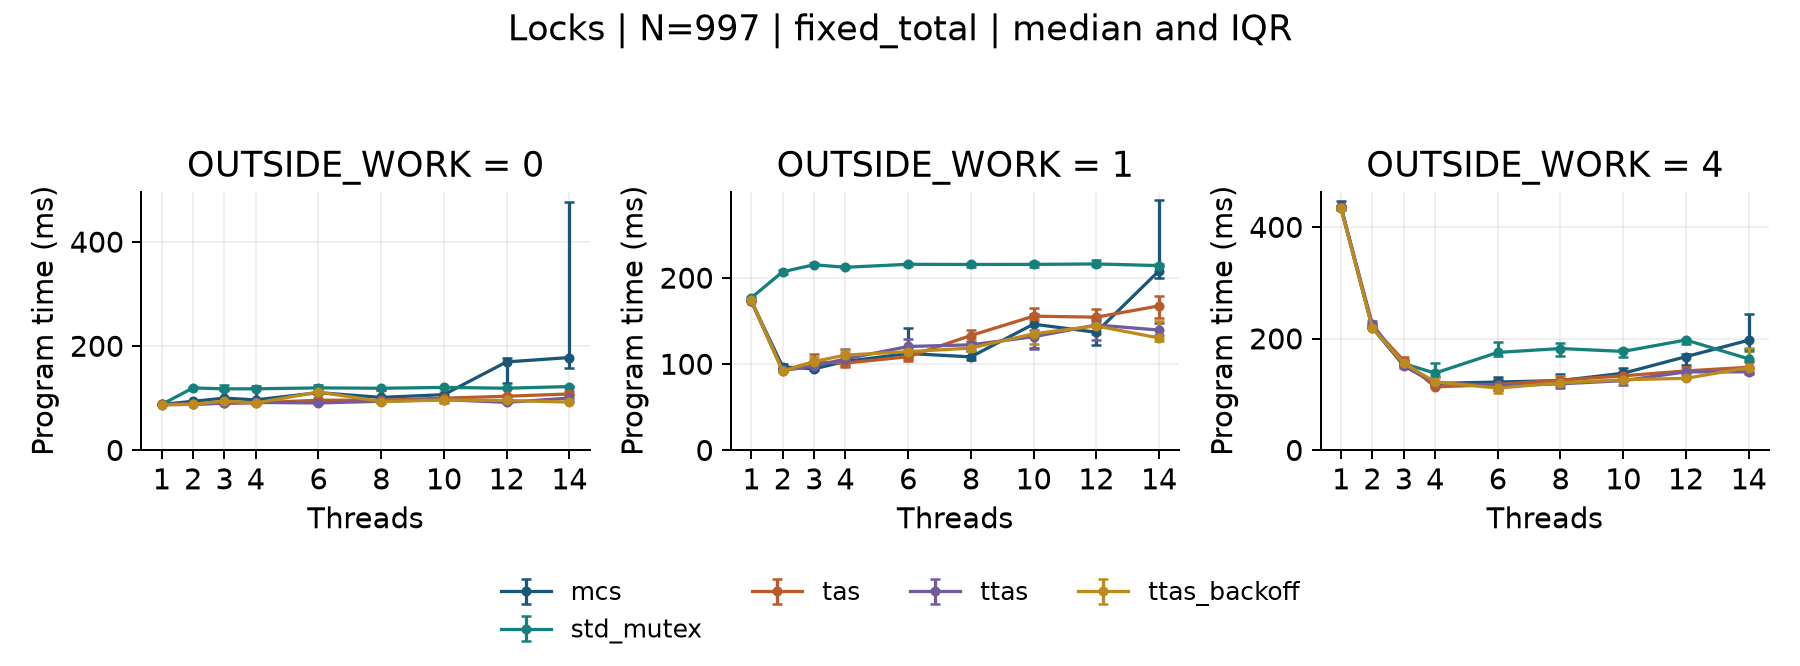
\includegraphics[width=\textwidth]{figures/locks_fixed_total.png}
\caption{Lock program time, fixed total $K=20000$, $N=997$, for $W=0,1,4$ (median and IQR).}\label{fig:locks-fixed}
\end{figure}

\textbf{All work inside the lock ($W=0$).} Equation~\eqref{eq:amdahl} allows no speedup, so the best a lock can do is to keep $T(P)$ at $T(1)\approx87.6$~ms (Table~\ref{tab:locks-fixed-w0}). TAS, TTAS and TTAS-backoff stay between 87 and 112~ms up to $P=14$. \texttt{std::mutex} rises to 119~ms as soon as $P=2$ and then stays flat. MCS stays within 26\% of $T(1)$ up to $P=10$ and climbs to 169--178~ms at $P=12$--14.

\begin{table}[H]
\centering
\footnotesize
\setlength{\tabcolsep}{3pt}
\caption{Median program time (ms), fixed total $K=20000$, $N=997$, $W=0$. Bold: fastest at each $P$.}\label{tab:locks-fixed-w0}
\begin{tabular}{|>{\raggedright\arraybackslash}p{\dimexpr 0.200\textwidth-2\tabcolsep-\arrayrulewidth\relax}|>{\raggedleft\arraybackslash}p{\dimexpr 0.088\textwidth-2\tabcolsep-\arrayrulewidth\relax}|>{\raggedleft\arraybackslash}p{\dimexpr 0.088\textwidth-2\tabcolsep-\arrayrulewidth\relax}|>{\raggedleft\arraybackslash}p{\dimexpr 0.088\textwidth-2\tabcolsep-\arrayrulewidth\relax}|>{\raggedleft\arraybackslash}p{\dimexpr 0.088\textwidth-2\tabcolsep-\arrayrulewidth\relax}|>{\raggedleft\arraybackslash}p{\dimexpr 0.088\textwidth-2\tabcolsep-\arrayrulewidth\relax}|>{\raggedleft\arraybackslash}p{\dimexpr 0.088\textwidth-2\tabcolsep-\arrayrulewidth\relax}|>{\raggedleft\arraybackslash}p{\dimexpr 0.088\textwidth-2\tabcolsep-\arrayrulewidth\relax}|>{\raggedleft\arraybackslash}p{\dimexpr 0.088\textwidth-2\tabcolsep-\arrayrulewidth\relax}|>{\raggedleft\arraybackslash}p{\dimexpr 0.088\textwidth-2\tabcolsep-\arrayrulewidth\relax}|}
\hline
\textbf{Lock (ms)} & \textbf{P=1} & \textbf{P=2} & \textbf{P=3} & \textbf{P=4} & \textbf{P=6} & \textbf{P=8} & \textbf{P=10} & \textbf{P=12} & \textbf{P=14} \\ \hline
\texttt{tas} & 87.5 & 88.5 & 90.1 & 90.7 & 95.7 & 95.6 & 99.6 & 103.4 & 107.7 \\ \hline
\texttt{ttas} & 87.3 & \textbf{87.7} & \textbf{90.0} & 91.5 & \textbf{90.4} & 93.7 & 96.9 & \textbf{91.6} & 99.8 \\ \hline
\texttt{ttas\_backoff} & \textbf{86.8} & 87.9 & 94.1 & \textbf{90.3} & 111.5 & \textbf{93.1} & \textbf{96.1} & 95.3 & \textbf{92.1} \\ \hline
\texttt{mcs} & 87.6 & 93.6 & 99.7 & 96.3 & 110.2 & 101.1 & 106.4 & 169.3 & 177.6 \\ \hline
\texttt{std\_mutex} & 87.6 & 119.3 & 117.6 & 117.6 & 119.4 & 118.7 & 120.3 & 118.8 & 121.9 \\ \hline
\end{tabular}
\end{table}


\textbf{Work outside the lock ($W>0$).} Now the threads can overlap their outside calls, and Table~\ref{tab:speedup-w4} shows how close each lock comes to the bound $S\le W+1$. At $W=1$ the spinlocks reach 1.9$\times$ at $P=2$, close to the bound of 2. At $W=4$ (bound 5) the best speedup is 3.9$\times$ (TTAS-backoff, $P=6$), and at $W=8$ (bound 9) it is 5.6$\times$ (TAS, $P=12$; Table~\ref{tab:speedup-w8}). The gap to the bound grows with $W$ because more threads are needed to approach it, and more threads contend for the lock at every release.

\begin{table}[H]
\centering
\footnotesize
\setlength{\tabcolsep}{3pt}
\caption{Speedup $S(P)=T(1)/T(P)$, fixed total, $N=997$, $W=4$ (Amdahl bound 5$\times$). Bold: highest at each $P$.}\label{tab:speedup-w4}
\begin{tabular}{|>{\raggedright\arraybackslash}p{\dimexpr 0.200\textwidth-2\tabcolsep-\arrayrulewidth\relax}|>{\raggedleft\arraybackslash}p{\dimexpr 0.099\textwidth-2\tabcolsep-\arrayrulewidth\relax}|>{\raggedleft\arraybackslash}p{\dimexpr 0.099\textwidth-2\tabcolsep-\arrayrulewidth\relax}|>{\raggedleft\arraybackslash}p{\dimexpr 0.099\textwidth-2\tabcolsep-\arrayrulewidth\relax}|>{\raggedleft\arraybackslash}p{\dimexpr 0.099\textwidth-2\tabcolsep-\arrayrulewidth\relax}|>{\raggedleft\arraybackslash}p{\dimexpr 0.099\textwidth-2\tabcolsep-\arrayrulewidth\relax}|>{\raggedleft\arraybackslash}p{\dimexpr 0.099\textwidth-2\tabcolsep-\arrayrulewidth\relax}|>{\raggedleft\arraybackslash}p{\dimexpr 0.099\textwidth-2\tabcolsep-\arrayrulewidth\relax}|>{\raggedleft\arraybackslash}p{\dimexpr 0.099\textwidth-2\tabcolsep-\arrayrulewidth\relax}|}
\hline
\textbf{Lock} & \textbf{P=2} & \textbf{P=3} & \textbf{P=4} & \textbf{P=6} & \textbf{P=8} & \textbf{P=10} & \textbf{P=12} & \textbf{P=14} \\ \hline
\texttt{tas} & 1.97 & 2.72 & \textbf{3.84} & 3.71 & 3.47 & 3.27 & 3.07 & 2.93 \\ \hline
\texttt{ttas} & 1.92 & 2.88 & 3.60 & 3.77 & \textbf{3.66} & \textbf{3.49} & 3.10 & \textbf{3.10} \\ \hline
\texttt{ttas\_backoff} & 1.98 & 2.79 & 3.55 & \textbf{3.90} & 3.60 & 3.44 & \textbf{3.37} & 2.93 \\ \hline
\texttt{mcs} & \textbf{1.99} & \textbf{2.88} & 3.66 & 3.58 & 3.51 & 3.17 & 2.61 & 2.22 \\ \hline
\texttt{std\_mutex} & 1.97 & 2.80 & 3.14 & 2.48 & 2.38 & 2.45 & 2.20 & 2.65 \\ \hline
\end{tabular}
\end{table}

\begin{table}[H]
\centering
\footnotesize
\setlength{\tabcolsep}{3pt}
\caption{Speedup $S(P)=T(1)/T(P)$, fixed total, $N=997$, $W=8$ (Amdahl bound 9$\times$). Bold: highest at each $P$.}\label{tab:speedup-w8}
\begin{tabular}{|>{\raggedright\arraybackslash}p{\dimexpr 0.200\textwidth-2\tabcolsep-\arrayrulewidth\relax}|>{\raggedleft\arraybackslash}p{\dimexpr 0.099\textwidth-2\tabcolsep-\arrayrulewidth\relax}|>{\raggedleft\arraybackslash}p{\dimexpr 0.099\textwidth-2\tabcolsep-\arrayrulewidth\relax}|>{\raggedleft\arraybackslash}p{\dimexpr 0.099\textwidth-2\tabcolsep-\arrayrulewidth\relax}|>{\raggedleft\arraybackslash}p{\dimexpr 0.099\textwidth-2\tabcolsep-\arrayrulewidth\relax}|>{\raggedleft\arraybackslash}p{\dimexpr 0.099\textwidth-2\tabcolsep-\arrayrulewidth\relax}|>{\raggedleft\arraybackslash}p{\dimexpr 0.099\textwidth-2\tabcolsep-\arrayrulewidth\relax}|>{\raggedleft\arraybackslash}p{\dimexpr 0.099\textwidth-2\tabcolsep-\arrayrulewidth\relax}|>{\raggedleft\arraybackslash}p{\dimexpr 0.099\textwidth-2\tabcolsep-\arrayrulewidth\relax}|}
\hline
\textbf{Lock} & \textbf{P=2} & \textbf{P=3} & \textbf{P=4} & \textbf{P=6} & \textbf{P=8} & \textbf{P=10} & \textbf{P=12} & \textbf{P=14} \\ \hline
\texttt{tas} & 1.96 & \textbf{2.91} & \textbf{3.88} & 4.30 & 4.88 & \textbf{5.41} & \textbf{5.65} & 4.95 \\ \hline
\texttt{ttas} & 1.95 & 2.90 & 3.69 & 3.91 & \textbf{5.20} & 5.33 & 5.57 & \textbf{5.45} \\ \hline
\texttt{ttas\_backoff} & 1.95 & 2.83 & 3.39 & 4.36 & 4.86 & 5.38 & 5.41 & 5.41 \\ \hline
\texttt{mcs} & 1.97 & 2.89 & 3.59 & \textbf{5.08} & 5.02 & 5.29 & 4.58 & 3.74 \\ \hline
\texttt{std\_mutex} & \textbf{1.99} & 2.90 & 3.67 & 3.29 & 3.20 & 3.26 & 3.22 & 3.15 \\ \hline
\end{tabular}
\end{table}


\textbf{Beyond 6 to 10 threads} every lock gets slower again (Figure~\ref{fig:locks-fixed}, right). More waiters compete for the lock's cache line at each release. In addition, the laptop has only 6 performance cores, so higher $P$ places threads on the efficiency cores and on Hyper-Threading siblings, which run the primality loop more slowly. This placement explanation is a hypothesis consistent with the data, not a measured scheduler trace.

\subsection{Cost of passing the lock}\label{sec:res-outside}

In per-thread mode every thread performs $I=5000$ iterations, so the total work grows with $P$ (Figure~\ref{fig:locks-per-thread}); this is the statement's program as given. With $W=0$ all of that work is serial, so $T(P)\ge P\cdot T(1)$, and the ratio $T(P)/(P\cdot T(1))$ measures what each lock adds on top of the serial work, mainly the cost of passing ownership from one thread to the next. Computed from Table~\ref{tab:locks-per-thread-w0}, the ratio at $P=14$ is 1.03 for TTAS, 1.06 for TTAS-backoff, 1.18 for TAS, 1.34 for \texttt{std::mutex} and 1.64 for MCS. \texttt{std::mutex} costs 1.33--1.35 at every $P$ from 2 to 14, a fixed price per handoff; TAS and MCS start near 1.0 and grow with $P$, which is the signature of contention.

\begin{figure}[H]
\centering
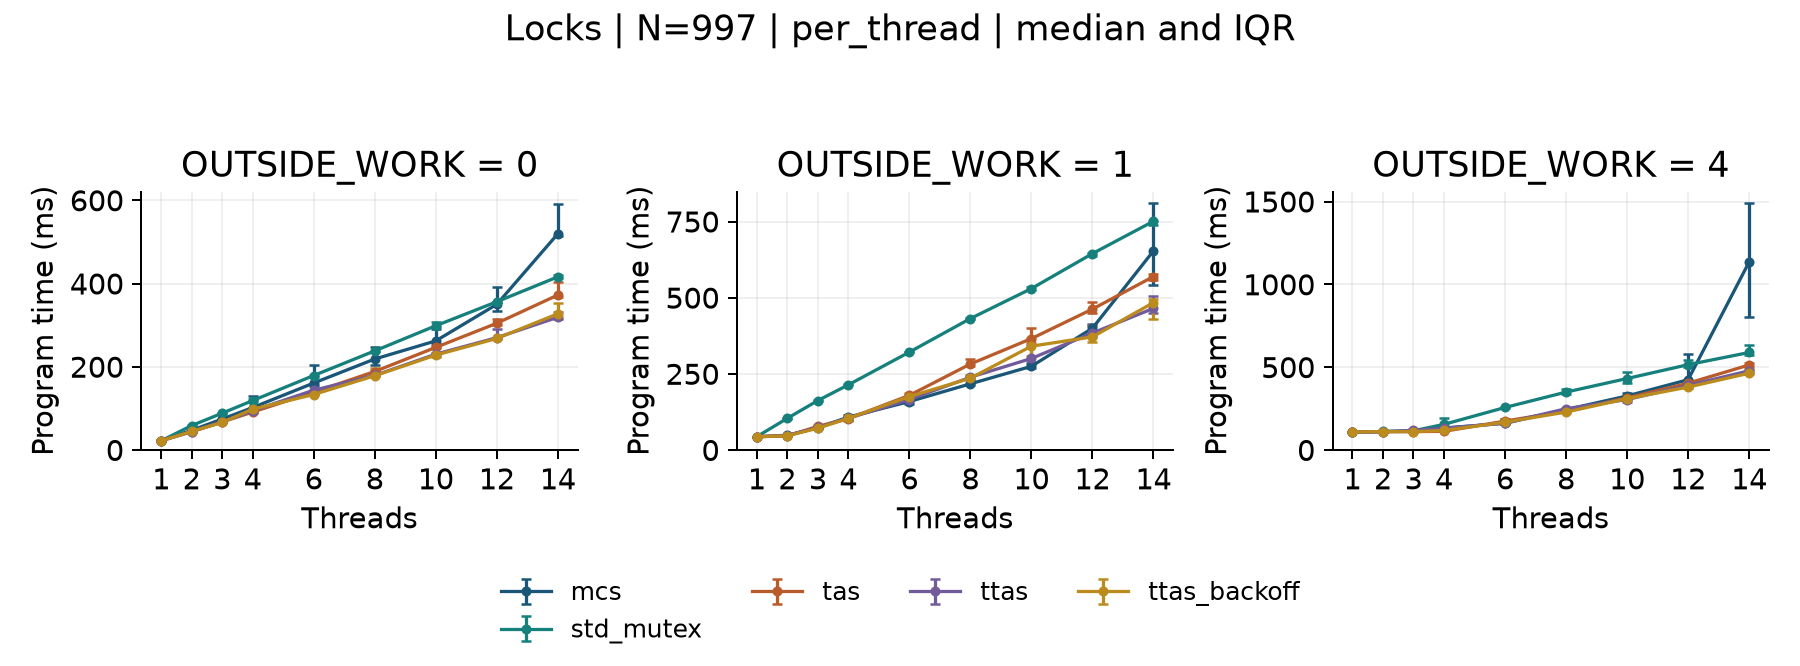
\includegraphics[width=\textwidth]{figures/locks_per_thread.png}
\caption{Lock program time, per-thread $I=5000$, $N=997$, for $W=0,1,4$; total work grows with $P$.}\label{fig:locks-per-thread}
\end{figure}

\subsection{Length of the critical section}\label{sec:res-sensitivity}

Figure~\ref{fig:locks-sens} changes $N$ to make each critical section about ten times shorter ($N=97$) or longer ($N=10007$). With short critical sections the lock changes owner very often. TAS then degrades from 82~ms at $P=1$ to 244~ms at $P=14$, because every waiter keeps executing \texttt{test\_and\_set} on the shared line, while TTAS, which waits with plain reads, stays at 89--106~ms for $P=2$--14 (Table~\ref{tab:sens-n97-w0}). This is the difference between TAS and TTAS that the slides predict, and it appears only when handoffs are frequent: with long critical sections all locks stay within 87--115~ms except MCS at $P=14$ (225~ms).

\begin{figure}[H]
\centering
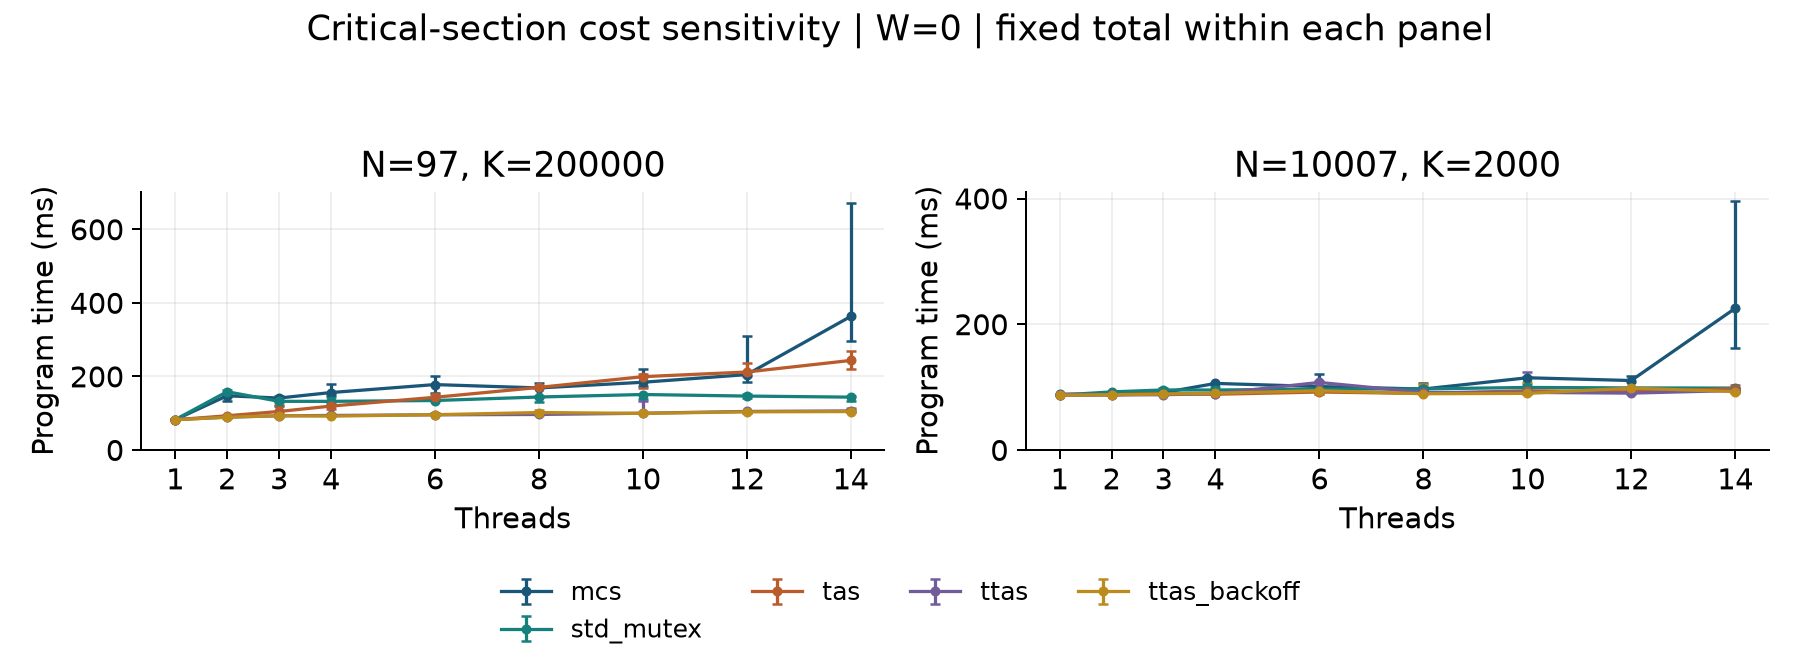
\includegraphics[width=\textwidth]{figures/locks_sensitivity.png}
\caption{Short ($N=97$, $K=200000$) and long ($N=10007$, $K=2000$) critical sections, $W=0$.}\label{fig:locks-sens}
\end{figure}

\subsection{Saturating every logical CPU}\label{sec:res-saturation}

Table~\ref{tab:saturation-locks} adds $P=15$ and 16. TAS, TTAS, TTAS-backoff and \texttt{std::mutex} stay at 91--122~ms at every $P$. MCS rises from 116~ms at $P=12$ to 333~ms at $P=15$ and 2468~ms at $P=16$, and its third quartile at $P=16$ is 61~s (Table~\ref{tab:saturation-locks-q3}); single runs at $P=16$ ranged from 0.18~s to 85~s. In the main run, one MCS warm-up at $P=14$ also exceeded 60~s.

\begin{table}[H]
\centering
\footnotesize
\setlength{\tabcolsep}{3pt}
\caption{Saturation run: median program time (ms), $N=997$, $W=0$, $K=20000$, five measured runs. Bold: fastest at each $P$.}\label{tab:saturation-locks}
\begin{tabular}{|>{\raggedright\arraybackslash}p{\dimexpr 0.200\textwidth-2\tabcolsep-\arrayrulewidth\relax}|>{\raggedleft\arraybackslash}p{\dimexpr 0.199\textwidth-2\tabcolsep-\arrayrulewidth\relax}|>{\raggedleft\arraybackslash}p{\dimexpr 0.199\textwidth-2\tabcolsep-\arrayrulewidth\relax}|>{\raggedleft\arraybackslash}p{\dimexpr 0.199\textwidth-2\tabcolsep-\arrayrulewidth\relax}|>{\raggedleft\arraybackslash}p{\dimexpr 0.199\textwidth-2\tabcolsep-\arrayrulewidth\relax}|}
\hline
\textbf{Lock (ms)} & \textbf{P=12} & \textbf{P=14} & \textbf{P=15} & \textbf{P=16} \\ \hline
\texttt{tas} & 107.4 & 113.2 & 108.5 & 109.0 \\ \hline
\texttt{ttas} & 97.4 & 98.1 & \textbf{104.3} & \textbf{102.5} \\ \hline
\texttt{ttas\_backoff} & \textbf{96.8} & \textbf{91.4} & 117.2 & 113.5 \\ \hline
\texttt{mcs} & 116.3 & 160.1 & 333.4 & 2\,468.2 \\ \hline
\texttt{std\_mutex} & 119.9 & 121.9 & 121.1 & 121.6 \\ \hline
\end{tabular}
\end{table}


MCS passes the lock to one specific thread, its queue successor. When the spinning threads occupy all 16 logical CPUs, together with the operating system's own threads, the scheduler must preempt some of them. If it preempts the successor, the lock is handed to a thread that is not running, and no thread can enter the critical section until the scheduler runs that thread again. This is the drawback the slides note for blocking objects and queue locks: a delayed thread delays all others. TAS and TTAS do not depend on any particular thread: whichever running thread wins the flag enters. The FIFO guarantee that makes MCS fair is thus what makes it fragile once threads outnumber free CPUs.

\subsection{Effect of exponential backoff}\label{sec:res-backoff}

TTAS with backoff helps where failed attempts are frequent. With short critical sections and $W=4$ it lowers the median from 160 to 144~ms at $P=4$ and from 246 to 226~ms at $P=14$ (Table~\ref{tab:sens-n97-w4}), and it gives the best speedups at $W=1$, 2 and 4. Elsewhere TTAS and TTAS-backoff are within each other's IQR, for example 99.8 against 92.1~ms at $P=14$, $W=0$. Backoff therefore never hurt noticeably in these experiments, but its gains are modest because TTAS already avoids most failed RMWs by waiting with reads. Its effect on the CAS counter is much larger (Section~\ref{sec:res-counters}).

\subsection{Comparison with \texttt{std::mutex}}\label{sec:res-stdmutex}

The statement asks for a comparison with existing mutex locks\cite{r1}; \texttt{std::mutex} of the C++ standard library (here libstdc++ for MinGW-w64) is measured in every experiment. It has the most predictable cost, a nearly constant 34\% over the serial bound in Section~\ref{sec:res-outside}, about 1.6~$\mu$s more per handoff than TTAS at $P=2$, $W=0$ (119.3 against 87.7~ms for 20000 handoffs). Because of that cost it never benefits from parallelism at $W=1$: it is slower than one thread for every $P$ from 2 to 14 (207--216 against 177~ms, Table~\ref{tab:locks-fixed-w1}), while the spinlocks almost halve the time. Its best speedup is 3.1$\times$ at $W=4$ and 3.7$\times$ at $W=8$, against 3.9$\times$ and 5.6$\times$ for the best spinlock. On the other hand, it is immune to the collapse of Section~\ref{sec:res-saturation}, because a blocked waiter sleeps instead of occupying a CPU. The likely reason for the handoff cost is that a waiting thread is woken through the operating system; this is a hypothesis, since the mutex's internals were not instrumented.

\subsection{Barrier throughput}\label{sec:res-barrier}

Figure~\ref{fig:barriers} and Table~\ref{tab:barriers} compare the sense-reversing barrier with \texttt{std::barrier}.

\begin{figure}[H]
\centering
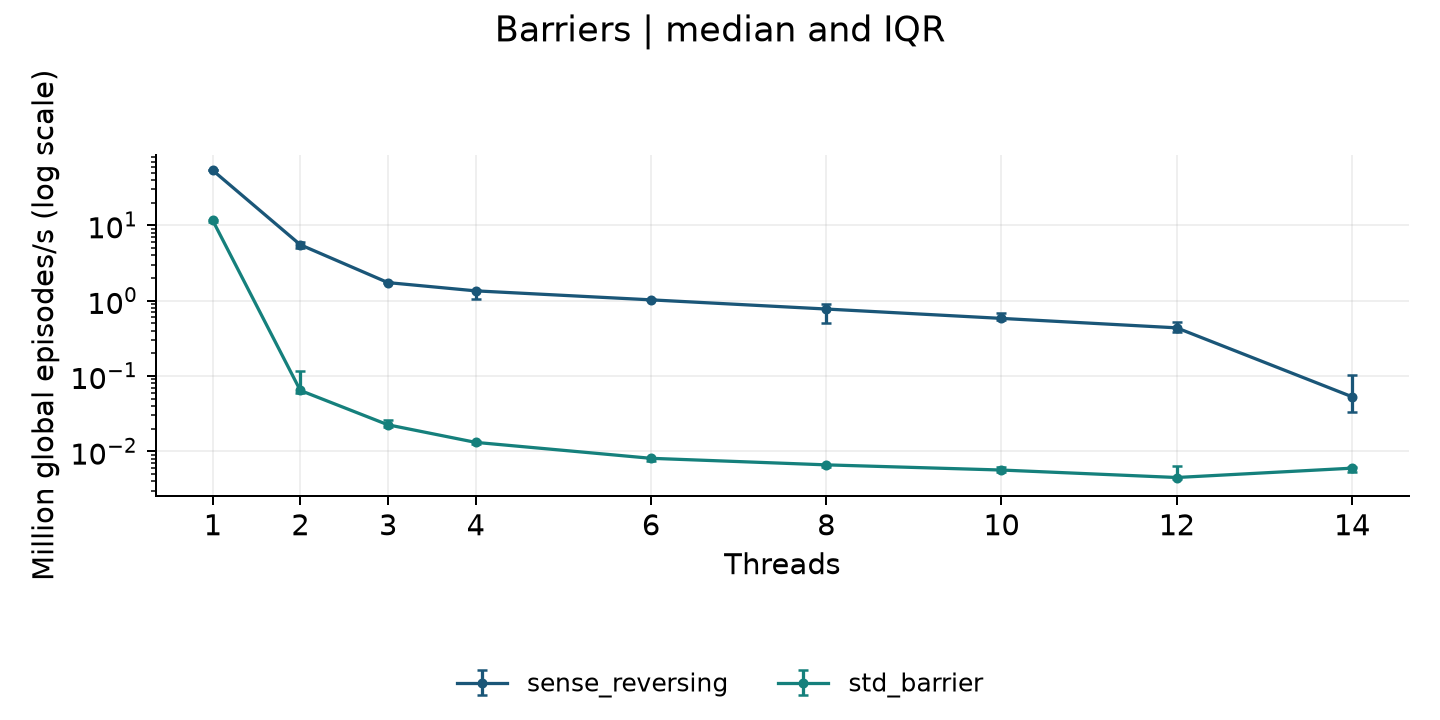
\includegraphics[width=0.85\textwidth]{figures/barriers.png}
\caption{Global barrier episodes per second, $E=20000$, no work between episodes (log scale).}\label{fig:barriers}
\end{figure}

\begin{table}[H]
\centering
\footnotesize
\setlength{\tabcolsep}{3pt}
\caption{Median global barrier episodes per second (thousands), $E=20000$, no work between episodes. Bold: highest at each $P$.}\label{tab:barriers}
\begin{tabular}{|>{\raggedright\arraybackslash}p{\dimexpr 0.200\textwidth-2\tabcolsep-\arrayrulewidth\relax}|>{\raggedleft\arraybackslash}p{\dimexpr 0.088\textwidth-2\tabcolsep-\arrayrulewidth\relax}|>{\raggedleft\arraybackslash}p{\dimexpr 0.088\textwidth-2\tabcolsep-\arrayrulewidth\relax}|>{\raggedleft\arraybackslash}p{\dimexpr 0.088\textwidth-2\tabcolsep-\arrayrulewidth\relax}|>{\raggedleft\arraybackslash}p{\dimexpr 0.088\textwidth-2\tabcolsep-\arrayrulewidth\relax}|>{\raggedleft\arraybackslash}p{\dimexpr 0.088\textwidth-2\tabcolsep-\arrayrulewidth\relax}|>{\raggedleft\arraybackslash}p{\dimexpr 0.088\textwidth-2\tabcolsep-\arrayrulewidth\relax}|>{\raggedleft\arraybackslash}p{\dimexpr 0.088\textwidth-2\tabcolsep-\arrayrulewidth\relax}|>{\raggedleft\arraybackslash}p{\dimexpr 0.088\textwidth-2\tabcolsep-\arrayrulewidth\relax}|>{\raggedleft\arraybackslash}p{\dimexpr 0.088\textwidth-2\tabcolsep-\arrayrulewidth\relax}|}
\hline
\textbf{Barrier (k/s)} & \textbf{P=1} & \textbf{P=2} & \textbf{P=3} & \textbf{P=4} & \textbf{P=6} & \textbf{P=8} & \textbf{P=10} & \textbf{P=12} & \textbf{P=14} \\ \hline
\texttt{sense\_reversing} & \textbf{53\,648} & \textbf{5\,510.2} & \textbf{1\,734.2} & \textbf{1\,348.0} & \textbf{1\,024.0} & \textbf{773.6} & \textbf{581.0} & \textbf{435.2} & \textbf{53.0} \\ \hline
\texttt{std\_barrier} & 11\,634 & 64.3 & 22.5 & 13.1 & 8.1 & 6.6 & 5.6 & 4.5 & 6.0 \\ \hline
\end{tabular}
\end{table}


At $P=1$ a barrier synchronizes nothing, so 54 million episodes per second only measure the cost of one call. From $P=2$ on, the sense-reversing barrier completes 5.5 million episodes per second against 64 thousand for \texttt{std::barrier}, and 435 thousand against 4.5 thousand at $P=12$: about two orders of magnitude. The sense-reversing barrier releases all waiters with one store to the sense flag, which each waiter sees in its spinning load. \texttt{std::barrier} in the GNU implementation is designed to let a waiting thread block after a short spin, so an episode can include operating-system wake-ups; its rate, nearly flat at 4.5--6.6 thousand per second from $P=8$ to 16, is consistent with a wake-up-bound cost.

The rate of the sense-reversing barrier falls as $P$ grows, because all arrivals perform an RMW on the same counter and the last thread must reach the barrier before anyone leaves. At $P=14$ it drops to 53 thousand per second in the main run and 127 thousand in the saturation run (Table~\ref{tab:saturation-barriers}), and to 22 thousand at $P=16$, still 3.7 times faster than \texttt{std::barrier}. A busy-waiting barrier depends on every participant running: one preempted thread stalls the whole episode. The difference between the two runs at $P=14$ shows how sensitive this regime is to the scheduler.

\begin{table}[H]
\centering
\footnotesize
\setlength{\tabcolsep}{3pt}
\caption{Saturation run: median global episodes per second (thousands). Bold: highest at each $P$.}\label{tab:saturation-barriers}
\begin{tabular}{|>{\raggedright\arraybackslash}p{\dimexpr 0.200\textwidth-2\tabcolsep-\arrayrulewidth\relax}|>{\raggedleft\arraybackslash}p{\dimexpr 0.199\textwidth-2\tabcolsep-\arrayrulewidth\relax}|>{\raggedleft\arraybackslash}p{\dimexpr 0.199\textwidth-2\tabcolsep-\arrayrulewidth\relax}|>{\raggedleft\arraybackslash}p{\dimexpr 0.199\textwidth-2\tabcolsep-\arrayrulewidth\relax}|>{\raggedleft\arraybackslash}p{\dimexpr 0.199\textwidth-2\tabcolsep-\arrayrulewidth\relax}|}
\hline
\textbf{Barrier (k/s)} & \textbf{P=12} & \textbf{P=14} & \textbf{P=15} & \textbf{P=16} \\ \hline
\texttt{sense\_reversing} & \textbf{426.3} & \textbf{127.4} & \textbf{112.6} & \textbf{22.3} \\ \hline
\texttt{std\_barrier} & 6.2 & 6.1 & 6.0 & 6.1 \\ \hline
\end{tabular}
\end{table}


\subsection{Concurrent counters}\label{sec:res-counters}

Figure~\ref{fig:counters} and Table~\ref{tab:counters} show the time for $K=1000000$ increments in total.

\begin{figure}[H]
\centering
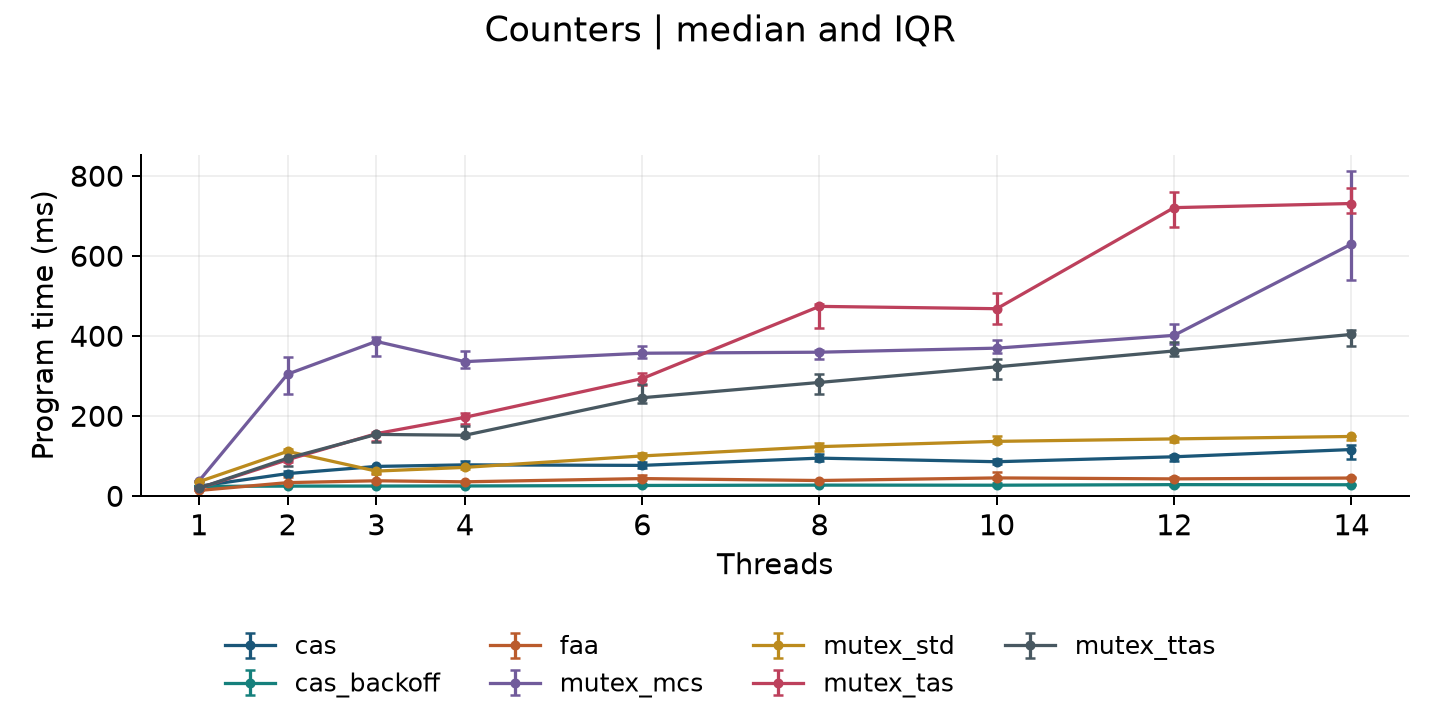
\includegraphics[width=0.85\textwidth]{figures/counters.png}
\caption{Counter program time for $K=1000000$ increments in total (median and IQR).}\label{fig:counters}
\end{figure}

\begin{table}[H]
\centering
\footnotesize
\setlength{\tabcolsep}{3pt}
\caption{Median program time (ms) for $K=1000000$ increments in total. Bold: fastest at each $P$.}\label{tab:counters}
\begin{tabular}{|>{\raggedright\arraybackslash}p{\dimexpr 0.200\textwidth-2\tabcolsep-\arrayrulewidth\relax}|>{\raggedleft\arraybackslash}p{\dimexpr 0.088\textwidth-2\tabcolsep-\arrayrulewidth\relax}|>{\raggedleft\arraybackslash}p{\dimexpr 0.088\textwidth-2\tabcolsep-\arrayrulewidth\relax}|>{\raggedleft\arraybackslash}p{\dimexpr 0.088\textwidth-2\tabcolsep-\arrayrulewidth\relax}|>{\raggedleft\arraybackslash}p{\dimexpr 0.088\textwidth-2\tabcolsep-\arrayrulewidth\relax}|>{\raggedleft\arraybackslash}p{\dimexpr 0.088\textwidth-2\tabcolsep-\arrayrulewidth\relax}|>{\raggedleft\arraybackslash}p{\dimexpr 0.088\textwidth-2\tabcolsep-\arrayrulewidth\relax}|>{\raggedleft\arraybackslash}p{\dimexpr 0.088\textwidth-2\tabcolsep-\arrayrulewidth\relax}|>{\raggedleft\arraybackslash}p{\dimexpr 0.088\textwidth-2\tabcolsep-\arrayrulewidth\relax}|>{\raggedleft\arraybackslash}p{\dimexpr 0.088\textwidth-2\tabcolsep-\arrayrulewidth\relax}|}
\hline
\textbf{Counter (ms)} & \textbf{P=1} & \textbf{P=2} & \textbf{P=3} & \textbf{P=4} & \textbf{P=6} & \textbf{P=8} & \textbf{P=10} & \textbf{P=12} & \textbf{P=14} \\ \hline
\texttt{mutex\_tas} & 19.5 & 90.5 & 155.6 & 196.6 & 293.4 & 473.8 & 468.0 & 720.6 & 731.0 \\ \hline
\texttt{mutex\_ttas} & 19.4 & 94.3 & 153.8 & 151.7 & 245.5 & 283.7 & 322.8 & 362.4 & 403.7 \\ \hline
\texttt{mutex\_mcs} & 37.3 & 304.4 & 386.3 & 335.7 & 356.7 & 359.3 & 369.4 & 401.4 & 629.4 \\ \hline
\texttt{mutex\_std} & 35.6 & 111.4 & 62.1 & 71.4 & 100.0 & 123.2 & 136.4 & 142.6 & 148.7 \\ \hline
\texttt{cas} & 24.4 & 55.9 & 73.8 & 77.7 & 76.4 & 94.5 & 85.5 & 97.9 & 116.0 \\ \hline
\texttt{cas\_backoff} & 23.9 & \textbf{24.6} & \textbf{24.8} & \textbf{24.9} & \textbf{26.2} & \textbf{27.1} & \textbf{26.9} & \textbf{28.3} & \textbf{28.0} \\ \hline
\texttt{faa} & \textbf{13.7} & 33.3 & 37.9 & 35.3 & 43.4 & 38.6 & 45.1 & 42.7 & 44.8 \\ \hline
\end{tabular}
\end{table}


\textbf{No counter is faster with more threads.} The fastest result is FAA with one thread, 13.7~ms. Every increment must update the same cache line, so the increments are serialized in hardware whatever the algorithm, and with more threads the line also moves between cores on every increment. A shared counter is a serial bottleneck, not a parallel workload.

\textbf{CAS with backoff} stays at 24--28~ms for every $P$, the lowest time from $P=2$ on. After a failed CAS the losing threads pause, so the winner can complete many increments in a row while its core owns the cache line. This raises throughput but concentrates the work on one thread at a time; it does not make the counter fairer. \textbf{Plain CAS} rises from 24~ms to 116~ms at $P=14$, because every failed attempt still moves the line. \textbf{FAA} stays at 33--45~ms for $P\ge2$, since an increment is a single RMW that cannot fail.

\textbf{Lock-based counters} pay an acquire and a release per increment, and the critical section is a single addition, so the cost of passing the lock dominates. With $P=14$ the counter takes 149~ms with \texttt{std::mutex}, 404~ms with TTAS, 629~ms with MCS and 731~ms with TAS. MCS is already at 304~ms with two threads, against 37~ms with one, presumably because almost every increment then hands the lock to a thread on another core. The ranking also differs from the prime workload: with $W=0$ at $P=14$, TAS beats \texttt{std::mutex} (108 against 122~ms), but in the counter, whose critical section is a single addition, TAS is the slowest lock and \texttt{std::mutex} the fastest. A lock cannot be chosen without knowing the length of the critical section and the number of threads.

\subsection{Summary of findings}

\begin{table}[H]
\centering
\small
\caption{Main findings on the measured laptop.}\label{tab:findings}
\begin{tabular}{|>{\raggedright\arraybackslash}p{\dimexpr 0.25\textwidth-2\tabcolsep-\arrayrulewidth\relax}|>{\raggedright\arraybackslash}p{\dimexpr 0.745\textwidth-2\tabcolsep-\arrayrulewidth\relax}|}
\hline
\textbf{Topic} & \textbf{Finding} \\ \hline
Speedup bound & Spinlocks reach 1.9$\times$, 2.8$\times$, 3.9$\times$ and 5.6$\times$ for $W=1,2,4,8$, against Amdahl bounds of 2, 3, 5 and 9. \\ \hline
TAS vs.\ TTAS & TTAS's read-only waiting matters with frequent handoffs: 106 against 244~ms at $P=14$, $N=97$. \\ \hline
MCS & Competitive up to about 10 threads; collapses at $P=15$--16 because a preempted queue successor blocks the lock. \\ \hline
\texttt{std::mutex} & A constant handoff cost of about 34\% over the serial bound; slower than one thread at $W=1$; robust when threads exceed CPUs. \\ \hline
Backoff & Modest gains for TTAS; large gains for the CAS counter, by serializing the work. \\ \hline
Barrier & Sense reversal is about 100$\times$ faster than \texttt{std::barrier} up to 12 threads and still 3.7$\times$ at 16. \\ \hline
Counters & No variant scales; FAA is the fastest single-thread option, CAS with backoff the fastest multi-thread option. \\ \hline
\end{tabular}
\end{table}

\newpage
\section{Conclusion}\label{sec:conclusion}

\subsection{Summary}

This assignment implemented the TAS, TTAS and MCS spinlocks, a reusable sense-reversing barrier, and concurrent counters based on locks, CAS and FAA in C++20, following the algorithms of the lecture and the acquire/release discipline of the C++ memory model. Correctness was tested by invariant checks under many threads, directed tests for the rare MCS and barrier interleavings, SC reference variants, stress runs and three sanitizers; all checks passed, including ThreadSanitizer with zero race warnings. The performance study on the student's laptop shows that:

\begin{itemize}[leftmargin=1.5em]
  \item the speedup of the lock workload is bounded by the share of work outside the lock, and the spinlocks come close to that bound at low thread counts;
  \item TTAS's read-only waiting is what keeps it efficient under frequent handoffs, where TAS degrades;
  \item MCS is fair and competitive up to about 10 threads but collapses when spinning threads fill every logical CPU, because a preempted successor blocks its queue;
  \item \texttt{std::mutex} pays a constant handoff cost that makes it slower than a single thread when half of the work is in the lock, but it is robust when threads exceed CPUs;
  \item the spinning sense-reversing barrier is about two orders of magnitude faster than \texttt{std::barrier} while every participant has a CPU;
  \item a shared counter does not scale with any synchronization method, and backoff improves its throughput by serializing the work.
\end{itemize}

\subsection{Limitations}

The study uses one platform, a hybrid laptop CPU without thread pinning, so the scheduler and the two core types contribute to the variation, and background load was reduced but not eliminated. Hardware performance counters were not used, so explanations involving cache traffic, core placement or operating-system wake-ups are hypotheses consistent with the timings. Finite tests and sanitizers do not prove every interleaving. With 15 or 16 threads the spinning results are dominated by scheduling, so they were separated into a saturation study.

\subsection{Future work}\label{sec:future}

The optional distributed part\cite{r1} was not implemented. MPI-3 one-sided communication\cite{r7} offers the primitives needed for it: \texttt{MPI\_Compare\_and\_swap} and \texttt{MPI\_Fetch\_and\_op} correspond to CAS and FAA on a window, and an MCS-style lock can be built from them with each process spinning on a flag in its own window. Further directions on shared memory are pinning threads to performance cores to separate the effect of the hybrid CPU, adding a ticket lock, which is also FIFO and should therefore show the same sensitivity to preemption, as a test of the explanation in Section~\ref{sec:res-saturation}, and a combining-tree or dissemination barrier to remove the shared counter.


\newpage
\begingroup\sloppy
\begin{thebibliography}{7}
\addcontentsline{toc}{section}{References}
\bibitem{r1} T. V. Hoai and D. T. Dang, ``Parallel Computing, Assignment 1,'' Ho Chi Minh City University of Technology, course CO5133, Sep. 16, 2026.

\bibitem{r2} K. Fürlinger, ``Advanced Topics in Parallel Computing,'' lecture slides used in course CO5133.

\bibitem{r3} J. M. Mellor-Crummey and M. L. Scott, ``Algorithms for scalable synchronization on shared-memory multiprocessors,'' \textit{ACM Transactions on Computer Systems}, vol. 9, no. 1, pp. 21--65, 1991.

\bibitem{r4} M. Herlihy and N. Shavit, \textit{The Art of Multiprocessor Programming}, revised 1st ed. Waltham, MA, USA: Morgan Kaufmann, 2012.

\bibitem{r5} M. L. Scott, \textit{Shared-Memory Synchronization}, Synthesis Lectures on Computer Architecture. San Rafael, CA, USA: Morgan \& Claypool, 2013.

\bibitem{r6} G. M. Amdahl, ``Validity of the single processor approach to achieving large scale computing capabilities,'' in \textit{Proc. AFIPS Spring Joint Computer Conference}, 1967, pp. 483--485.

\bibitem{r7} Message Passing Interface Forum, \textit{MPI: A Message-Passing Interface Standard, Version 4.1}, Nov. 2023, ch. 12. [Online]. Available: \url{https://www.mpi-forum.org/docs/mpi-4.1/mpi41-report.pdf}
\end{thebibliography}
\endgroup


\appendix
\newpage
\section{Complete Result Tables}\label{app:tables}

The tables in this appendix are generated from \texttt{results/processed/summary.csv} by \texttt{scripts/latex\_tables.py}; no value is typed by hand.

\subsection{Locks, fixed total work}
\begin{table}[H]
\centering
\footnotesize
\setlength{\tabcolsep}{3pt}
\caption{Median program time (ms), fixed total $K=20000$, $N=997$, $W=1$. Bold: fastest at each $P$.}\label{tab:locks-fixed-w1}
\begin{tabular}{|>{\raggedright\arraybackslash}p{\dimexpr 0.200\textwidth-2\tabcolsep-\arrayrulewidth\relax}|>{\raggedleft\arraybackslash}p{\dimexpr 0.088\textwidth-2\tabcolsep-\arrayrulewidth\relax}|>{\raggedleft\arraybackslash}p{\dimexpr 0.088\textwidth-2\tabcolsep-\arrayrulewidth\relax}|>{\raggedleft\arraybackslash}p{\dimexpr 0.088\textwidth-2\tabcolsep-\arrayrulewidth\relax}|>{\raggedleft\arraybackslash}p{\dimexpr 0.088\textwidth-2\tabcolsep-\arrayrulewidth\relax}|>{\raggedleft\arraybackslash}p{\dimexpr 0.088\textwidth-2\tabcolsep-\arrayrulewidth\relax}|>{\raggedleft\arraybackslash}p{\dimexpr 0.088\textwidth-2\tabcolsep-\arrayrulewidth\relax}|>{\raggedleft\arraybackslash}p{\dimexpr 0.088\textwidth-2\tabcolsep-\arrayrulewidth\relax}|>{\raggedleft\arraybackslash}p{\dimexpr 0.088\textwidth-2\tabcolsep-\arrayrulewidth\relax}|>{\raggedleft\arraybackslash}p{\dimexpr 0.088\textwidth-2\tabcolsep-\arrayrulewidth\relax}|}
\hline
\textbf{Lock (ms)} & \textbf{P=1} & \textbf{P=2} & \textbf{P=3} & \textbf{P=4} & \textbf{P=6} & \textbf{P=8} & \textbf{P=10} & \textbf{P=12} & \textbf{P=14} \\ \hline
\texttt{tas} & \textbf{173.0} & 92.2 & 102.5 & \textbf{101.0} & \textbf{108.3} & 132.9 & 155.4 & 154.3 & 167.3 \\ \hline
\texttt{ttas} & 173.2 & 92.4 & 97.5 & 105.8 & 120.2 & 122.1 & \textbf{131.5} & 145.2 & 139.3 \\ \hline
\texttt{ttas\_backoff} & 174.2 & \textbf{91.4} & 102.8 & 110.2 & 114.3 & 118.3 & 135.0 & 144.1 & \textbf{130.1} \\ \hline
\texttt{mcs} & 173.1 & 96.6 & \textbf{94.3} & 102.8 & 112.1 & \textbf{108.2} & 146.1 & \textbf{136.7} & 207.9 \\ \hline
\texttt{std\_mutex} & 176.8 & 207.0 & 215.1 & 212.2 & 215.6 & 215.4 & 215.5 & 216.1 & 214.2 \\ \hline
\end{tabular}
\end{table}

\begin{table}[H]
\centering
\footnotesize
\setlength{\tabcolsep}{3pt}
\caption{Median program time (ms), fixed total $K=20000$, $N=997$, $W=2$. Bold: fastest at each $P$.}\label{tab:locks-fixed-w2}
\begin{tabular}{|>{\raggedright\arraybackslash}p{\dimexpr 0.200\textwidth-2\tabcolsep-\arrayrulewidth\relax}|>{\raggedleft\arraybackslash}p{\dimexpr 0.088\textwidth-2\tabcolsep-\arrayrulewidth\relax}|>{\raggedleft\arraybackslash}p{\dimexpr 0.088\textwidth-2\tabcolsep-\arrayrulewidth\relax}|>{\raggedleft\arraybackslash}p{\dimexpr 0.088\textwidth-2\tabcolsep-\arrayrulewidth\relax}|>{\raggedleft\arraybackslash}p{\dimexpr 0.088\textwidth-2\tabcolsep-\arrayrulewidth\relax}|>{\raggedleft\arraybackslash}p{\dimexpr 0.088\textwidth-2\tabcolsep-\arrayrulewidth\relax}|>{\raggedleft\arraybackslash}p{\dimexpr 0.088\textwidth-2\tabcolsep-\arrayrulewidth\relax}|>{\raggedleft\arraybackslash}p{\dimexpr 0.088\textwidth-2\tabcolsep-\arrayrulewidth\relax}|>{\raggedleft\arraybackslash}p{\dimexpr 0.088\textwidth-2\tabcolsep-\arrayrulewidth\relax}|>{\raggedleft\arraybackslash}p{\dimexpr 0.088\textwidth-2\tabcolsep-\arrayrulewidth\relax}|}
\hline
\textbf{Lock (ms)} & \textbf{P=1} & \textbf{P=2} & \textbf{P=3} & \textbf{P=4} & \textbf{P=6} & \textbf{P=8} & \textbf{P=10} & \textbf{P=12} & \textbf{P=14} \\ \hline
\texttt{tas} & 260.6 & 132.9 & 98.7 & 103.6 & 109.4 & 129.0 & 129.1 & 142.1 & 150.0 \\ \hline
\texttt{ttas} & \textbf{259.5} & \textbf{132.5} & 96.4 & 106.3 & 117.8 & 118.9 & \textbf{119.5} & 132.3 & \textbf{136.4} \\ \hline
\texttt{ttas\_backoff} & 262.0 & 132.9 & \textbf{94.0} & 105.7 & \textbf{105.0} & 123.1 & 123.3 & \textbf{126.7} & 138.5 \\ \hline
\texttt{mcs} & 259.7 & 133.2 & 97.3 & \textbf{95.3} & 106.0 & \textbf{115.5} & 142.9 & 176.1 & 290.8 \\ \hline
\texttt{std\_mutex} & 260.5 & 135.1 & 230.1 & 203.6 & 240.8 & 216.7 & 213.4 & 210.1 & 223.9 \\ \hline
\end{tabular}
\end{table}

\begin{table}[H]
\centering
\footnotesize
\setlength{\tabcolsep}{3pt}
\caption{Median program time (ms), fixed total $K=20000$, $N=997$, $W=4$. Bold: fastest at each $P$.}\label{tab:locks-fixed-w4}
\begin{tabular}{|>{\raggedright\arraybackslash}p{\dimexpr 0.200\textwidth-2\tabcolsep-\arrayrulewidth\relax}|>{\raggedleft\arraybackslash}p{\dimexpr 0.088\textwidth-2\tabcolsep-\arrayrulewidth\relax}|>{\raggedleft\arraybackslash}p{\dimexpr 0.088\textwidth-2\tabcolsep-\arrayrulewidth\relax}|>{\raggedleft\arraybackslash}p{\dimexpr 0.088\textwidth-2\tabcolsep-\arrayrulewidth\relax}|>{\raggedleft\arraybackslash}p{\dimexpr 0.088\textwidth-2\tabcolsep-\arrayrulewidth\relax}|>{\raggedleft\arraybackslash}p{\dimexpr 0.088\textwidth-2\tabcolsep-\arrayrulewidth\relax}|>{\raggedleft\arraybackslash}p{\dimexpr 0.088\textwidth-2\tabcolsep-\arrayrulewidth\relax}|>{\raggedleft\arraybackslash}p{\dimexpr 0.088\textwidth-2\tabcolsep-\arrayrulewidth\relax}|>{\raggedleft\arraybackslash}p{\dimexpr 0.088\textwidth-2\tabcolsep-\arrayrulewidth\relax}|>{\raggedleft\arraybackslash}p{\dimexpr 0.088\textwidth-2\tabcolsep-\arrayrulewidth\relax}|}
\hline
\textbf{Lock (ms)} & \textbf{P=1} & \textbf{P=2} & \textbf{P=3} & \textbf{P=4} & \textbf{P=6} & \textbf{P=8} & \textbf{P=10} & \textbf{P=12} & \textbf{P=14} \\ \hline
\texttt{tas} & 435.4 & 221.0 & 160.3 & \textbf{113.3} & 117.4 & 125.5 & 133.1 & 141.9 & 148.5 \\ \hline
\texttt{ttas} & 434.5 & 225.9 & \textbf{150.9} & 120.8 & 115.3 & \textbf{118.7} & \textbf{124.5} & 140.2 & \textbf{140.3} \\ \hline
\texttt{ttas\_backoff} & 433.7 & \textbf{219.3} & 155.7 & 122.0 & \textbf{111.2} & 120.5 & 126.1 & \textbf{128.6} & 147.8 \\ \hline
\texttt{mcs} & 437.1 & 219.5 & 151.6 & 119.5 & 122.0 & 124.6 & 137.7 & 167.4 & 196.9 \\ \hline
\texttt{std\_mutex} & \textbf{433.5} & 219.8 & 155.1 & 138.0 & 175.1 & 182.1 & 176.9 & 197.3 & 163.6 \\ \hline
\end{tabular}
\end{table}

\begin{table}[H]
\centering
\footnotesize
\setlength{\tabcolsep}{3pt}
\caption{Median program time (ms), fixed total $K=20000$, $N=997$, $W=8$. Bold: fastest at each $P$.}\label{tab:locks-fixed-w8}
\begin{tabular}{|>{\raggedright\arraybackslash}p{\dimexpr 0.200\textwidth-2\tabcolsep-\arrayrulewidth\relax}|>{\raggedleft\arraybackslash}p{\dimexpr 0.088\textwidth-2\tabcolsep-\arrayrulewidth\relax}|>{\raggedleft\arraybackslash}p{\dimexpr 0.088\textwidth-2\tabcolsep-\arrayrulewidth\relax}|>{\raggedleft\arraybackslash}p{\dimexpr 0.088\textwidth-2\tabcolsep-\arrayrulewidth\relax}|>{\raggedleft\arraybackslash}p{\dimexpr 0.088\textwidth-2\tabcolsep-\arrayrulewidth\relax}|>{\raggedleft\arraybackslash}p{\dimexpr 0.088\textwidth-2\tabcolsep-\arrayrulewidth\relax}|>{\raggedleft\arraybackslash}p{\dimexpr 0.088\textwidth-2\tabcolsep-\arrayrulewidth\relax}|>{\raggedleft\arraybackslash}p{\dimexpr 0.088\textwidth-2\tabcolsep-\arrayrulewidth\relax}|>{\raggedleft\arraybackslash}p{\dimexpr 0.088\textwidth-2\tabcolsep-\arrayrulewidth\relax}|>{\raggedleft\arraybackslash}p{\dimexpr 0.088\textwidth-2\tabcolsep-\arrayrulewidth\relax}|}
\hline
\textbf{Lock (ms)} & \textbf{P=1} & \textbf{P=2} & \textbf{P=3} & \textbf{P=4} & \textbf{P=6} & \textbf{P=8} & \textbf{P=10} & \textbf{P=12} & \textbf{P=14} \\ \hline
\texttt{tas} & 780.6 & 399.1 & \textbf{268.5} & \textbf{201.2} & 181.6 & 159.8 & \textbf{144.4} & \textbf{138.3} & 157.7 \\ \hline
\texttt{ttas} & \textbf{778.0} & 399.7 & 268.7 & 211.1 & 198.7 & \textbf{149.6} & 145.9 & 139.8 & \textbf{142.8} \\ \hline
\texttt{ttas\_backoff} & 779.3 & 400.4 & 275.8 & 230.2 & 178.7 & 160.3 & 144.8 & 144.0 & 143.9 \\ \hline
\texttt{mcs} & 778.3 & 395.1 & 269.3 & 216.5 & \textbf{153.2} & 155.0 & 147.2 & 169.9 & 208.1 \\ \hline
\texttt{std\_mutex} & 780.2 & \textbf{391.6} & 269.2 & 212.6 & 237.3 & 244.1 & 239.0 & 242.1 & 247.9 \\ \hline
\end{tabular}
\end{table}

\begin{table}[H]
\centering
\footnotesize
\setlength{\tabcolsep}{3pt}
\caption{Speedup $S(P)=T(1)/T(P)$, fixed total, $N=997$, $W=1$ (Amdahl bound 2$\times$). Bold: highest at each $P$.}\label{tab:speedup-w1}
\begin{tabular}{|>{\raggedright\arraybackslash}p{\dimexpr 0.200\textwidth-2\tabcolsep-\arrayrulewidth\relax}|>{\raggedleft\arraybackslash}p{\dimexpr 0.099\textwidth-2\tabcolsep-\arrayrulewidth\relax}|>{\raggedleft\arraybackslash}p{\dimexpr 0.099\textwidth-2\tabcolsep-\arrayrulewidth\relax}|>{\raggedleft\arraybackslash}p{\dimexpr 0.099\textwidth-2\tabcolsep-\arrayrulewidth\relax}|>{\raggedleft\arraybackslash}p{\dimexpr 0.099\textwidth-2\tabcolsep-\arrayrulewidth\relax}|>{\raggedleft\arraybackslash}p{\dimexpr 0.099\textwidth-2\tabcolsep-\arrayrulewidth\relax}|>{\raggedleft\arraybackslash}p{\dimexpr 0.099\textwidth-2\tabcolsep-\arrayrulewidth\relax}|>{\raggedleft\arraybackslash}p{\dimexpr 0.099\textwidth-2\tabcolsep-\arrayrulewidth\relax}|>{\raggedleft\arraybackslash}p{\dimexpr 0.099\textwidth-2\tabcolsep-\arrayrulewidth\relax}|}
\hline
\textbf{Lock} & \textbf{P=2} & \textbf{P=3} & \textbf{P=4} & \textbf{P=6} & \textbf{P=8} & \textbf{P=10} & \textbf{P=12} & \textbf{P=14} \\ \hline
\texttt{tas} & 1.88 & 1.69 & \textbf{1.71} & \textbf{1.60} & 1.30 & 1.11 & 1.12 & 1.03 \\ \hline
\texttt{ttas} & 1.88 & 1.78 & 1.64 & 1.44 & 1.42 & \textbf{1.32} & 1.19 & 1.24 \\ \hline
\texttt{ttas\_backoff} & \textbf{1.91} & 1.69 & 1.58 & 1.52 & 1.47 & 1.29 & 1.21 & \textbf{1.34} \\ \hline
\texttt{mcs} & 1.79 & \textbf{1.84} & 1.68 & 1.54 & \textbf{1.60} & 1.18 & \textbf{1.27} & 0.83 \\ \hline
\texttt{std\_mutex} & 0.85 & 0.82 & 0.83 & 0.82 & 0.82 & 0.82 & 0.82 & 0.83 \\ \hline
\end{tabular}
\end{table}

\begin{table}[H]
\centering
\footnotesize
\setlength{\tabcolsep}{3pt}
\caption{Speedup $S(P)=T(1)/T(P)$, fixed total, $N=997$, $W=2$ (Amdahl bound 3$\times$). Bold: highest at each $P$.}\label{tab:speedup-w2}
\begin{tabular}{|>{\raggedright\arraybackslash}p{\dimexpr 0.200\textwidth-2\tabcolsep-\arrayrulewidth\relax}|>{\raggedleft\arraybackslash}p{\dimexpr 0.099\textwidth-2\tabcolsep-\arrayrulewidth\relax}|>{\raggedleft\arraybackslash}p{\dimexpr 0.099\textwidth-2\tabcolsep-\arrayrulewidth\relax}|>{\raggedleft\arraybackslash}p{\dimexpr 0.099\textwidth-2\tabcolsep-\arrayrulewidth\relax}|>{\raggedleft\arraybackslash}p{\dimexpr 0.099\textwidth-2\tabcolsep-\arrayrulewidth\relax}|>{\raggedleft\arraybackslash}p{\dimexpr 0.099\textwidth-2\tabcolsep-\arrayrulewidth\relax}|>{\raggedleft\arraybackslash}p{\dimexpr 0.099\textwidth-2\tabcolsep-\arrayrulewidth\relax}|>{\raggedleft\arraybackslash}p{\dimexpr 0.099\textwidth-2\tabcolsep-\arrayrulewidth\relax}|>{\raggedleft\arraybackslash}p{\dimexpr 0.099\textwidth-2\tabcolsep-\arrayrulewidth\relax}|}
\hline
\textbf{Lock} & \textbf{P=2} & \textbf{P=3} & \textbf{P=4} & \textbf{P=6} & \textbf{P=8} & \textbf{P=10} & \textbf{P=12} & \textbf{P=14} \\ \hline
\texttt{tas} & 1.96 & 2.64 & 2.52 & 2.38 & 2.02 & 2.02 & 1.83 & 1.74 \\ \hline
\texttt{ttas} & 1.96 & 2.69 & 2.44 & 2.20 & 2.18 & \textbf{2.17} & 1.96 & \textbf{1.90} \\ \hline
\texttt{ttas\_backoff} & \textbf{1.97} & \textbf{2.79} & 2.48 & \textbf{2.50} & 2.13 & 2.13 & \textbf{2.07} & 1.89 \\ \hline
\texttt{mcs} & 1.95 & 2.67 & \textbf{2.73} & 2.45 & \textbf{2.25} & 1.82 & 1.47 & 0.89 \\ \hline
\texttt{std\_mutex} & 1.93 & 1.13 & 1.28 & 1.08 & 1.20 & 1.22 & 1.24 & 1.16 \\ \hline
\end{tabular}
\end{table}


\subsection{Locks, per-thread work}
\begin{table}[H]
\centering
\footnotesize
\setlength{\tabcolsep}{3pt}
\caption{Median program time (ms), per-thread $I=5000$, $N=997$, $W=0$; total work grows with $P$.}\label{tab:locks-per-thread-w0}
\begin{tabular}{|>{\raggedright\arraybackslash}p{\dimexpr 0.200\textwidth-2\tabcolsep-\arrayrulewidth\relax}|>{\raggedleft\arraybackslash}p{\dimexpr 0.088\textwidth-2\tabcolsep-\arrayrulewidth\relax}|>{\raggedleft\arraybackslash}p{\dimexpr 0.088\textwidth-2\tabcolsep-\arrayrulewidth\relax}|>{\raggedleft\arraybackslash}p{\dimexpr 0.088\textwidth-2\tabcolsep-\arrayrulewidth\relax}|>{\raggedleft\arraybackslash}p{\dimexpr 0.088\textwidth-2\tabcolsep-\arrayrulewidth\relax}|>{\raggedleft\arraybackslash}p{\dimexpr 0.088\textwidth-2\tabcolsep-\arrayrulewidth\relax}|>{\raggedleft\arraybackslash}p{\dimexpr 0.088\textwidth-2\tabcolsep-\arrayrulewidth\relax}|>{\raggedleft\arraybackslash}p{\dimexpr 0.088\textwidth-2\tabcolsep-\arrayrulewidth\relax}|>{\raggedleft\arraybackslash}p{\dimexpr 0.088\textwidth-2\tabcolsep-\arrayrulewidth\relax}|>{\raggedleft\arraybackslash}p{\dimexpr 0.088\textwidth-2\tabcolsep-\arrayrulewidth\relax}|}
\hline
\textbf{Lock (ms)} & \textbf{P=1} & \textbf{P=2} & \textbf{P=3} & \textbf{P=4} & \textbf{P=6} & \textbf{P=8} & \textbf{P=10} & \textbf{P=12} & \textbf{P=14} \\ \hline
\texttt{tas} & 22.6 & \textbf{44.1} & 67.5 & \textbf{91.4} & 139.0 & 188.7 & 246.7 & 304.7 & 372.6 \\ \hline
\texttt{ttas} & 22.2 & 44.5 & 67.9 & 94.5 & 143.8 & 179.3 & 230.4 & 270.1 & \textbf{319.2} \\ \hline
\texttt{ttas\_backoff} & \textbf{22.1} & 44.7 & \textbf{66.4} & 98.2 & \textbf{133.5} & \textbf{178.6} & \textbf{228.2} & \textbf{268.1} & 327.5 \\ \hline
\texttt{mcs} & 22.7 & 47.4 & 74.5 & 102.1 & 161.0 & 218.8 & 262.3 & 350.1 & 519.7 \\ \hline
\texttt{std\_mutex} & 22.2 & 58.8 & 88.6 & 118.9 & 179.1 & 238.3 & 298.7 & 356.5 & 416.2 \\ \hline
\end{tabular}
\end{table}

\begin{table}[H]
\centering
\footnotesize
\setlength{\tabcolsep}{3pt}
\caption{Median program time (ms), per-thread $I=5000$, $N=997$, $W=1$; total work grows with $P$.}\label{tab:locks-per-thread-w1}
\begin{tabular}{|>{\raggedright\arraybackslash}p{\dimexpr 0.200\textwidth-2\tabcolsep-\arrayrulewidth\relax}|>{\raggedleft\arraybackslash}p{\dimexpr 0.088\textwidth-2\tabcolsep-\arrayrulewidth\relax}|>{\raggedleft\arraybackslash}p{\dimexpr 0.088\textwidth-2\tabcolsep-\arrayrulewidth\relax}|>{\raggedleft\arraybackslash}p{\dimexpr 0.088\textwidth-2\tabcolsep-\arrayrulewidth\relax}|>{\raggedleft\arraybackslash}p{\dimexpr 0.088\textwidth-2\tabcolsep-\arrayrulewidth\relax}|>{\raggedleft\arraybackslash}p{\dimexpr 0.088\textwidth-2\tabcolsep-\arrayrulewidth\relax}|>{\raggedleft\arraybackslash}p{\dimexpr 0.088\textwidth-2\tabcolsep-\arrayrulewidth\relax}|>{\raggedleft\arraybackslash}p{\dimexpr 0.088\textwidth-2\tabcolsep-\arrayrulewidth\relax}|>{\raggedleft\arraybackslash}p{\dimexpr 0.088\textwidth-2\tabcolsep-\arrayrulewidth\relax}|>{\raggedleft\arraybackslash}p{\dimexpr 0.088\textwidth-2\tabcolsep-\arrayrulewidth\relax}|}
\hline
\textbf{Lock (ms)} & \textbf{P=1} & \textbf{P=2} & \textbf{P=3} & \textbf{P=4} & \textbf{P=6} & \textbf{P=8} & \textbf{P=10} & \textbf{P=12} & \textbf{P=14} \\ \hline
\texttt{tas} & 43.8 & \textbf{46.5} & 77.8 & \textbf{103.2} & 179.5 & 282.5 & 365.9 & 462.8 & 569.6 \\ \hline
\texttt{ttas} & 43.7 & 47.3 & 74.2 & 104.4 & 165.8 & 239.1 & 300.7 & 384.2 & \textbf{465.2} \\ \hline
\texttt{ttas\_backoff} & 43.9 & 46.7 & \textbf{71.8} & 103.9 & 175.6 & 235.8 & 341.0 & \textbf{371.5} & 484.1 \\ \hline
\texttt{mcs} & \textbf{43.7} & 48.7 & 73.0 & 108.3 & \textbf{159.2} & \textbf{217.4} & \textbf{274.9} & 400.0 & 653.9 \\ \hline
\texttt{std\_mutex} & 43.9 & 104.1 & 162.5 & 214.1 & 321.6 & 431.7 & 530.2 & 645.0 & 751.2 \\ \hline
\end{tabular}
\end{table}

\begin{table}[H]
\centering
\footnotesize
\setlength{\tabcolsep}{3pt}
\caption{Median program time (ms), per-thread $I=5000$, $N=997$, $W=2$; total work grows with $P$.}\label{tab:locks-per-thread-w2}
\begin{tabular}{|>{\raggedright\arraybackslash}p{\dimexpr 0.200\textwidth-2\tabcolsep-\arrayrulewidth\relax}|>{\raggedleft\arraybackslash}p{\dimexpr 0.088\textwidth-2\tabcolsep-\arrayrulewidth\relax}|>{\raggedleft\arraybackslash}p{\dimexpr 0.088\textwidth-2\tabcolsep-\arrayrulewidth\relax}|>{\raggedleft\arraybackslash}p{\dimexpr 0.088\textwidth-2\tabcolsep-\arrayrulewidth\relax}|>{\raggedleft\arraybackslash}p{\dimexpr 0.088\textwidth-2\tabcolsep-\arrayrulewidth\relax}|>{\raggedleft\arraybackslash}p{\dimexpr 0.088\textwidth-2\tabcolsep-\arrayrulewidth\relax}|>{\raggedleft\arraybackslash}p{\dimexpr 0.088\textwidth-2\tabcolsep-\arrayrulewidth\relax}|>{\raggedleft\arraybackslash}p{\dimexpr 0.088\textwidth-2\tabcolsep-\arrayrulewidth\relax}|>{\raggedleft\arraybackslash}p{\dimexpr 0.088\textwidth-2\tabcolsep-\arrayrulewidth\relax}|>{\raggedleft\arraybackslash}p{\dimexpr 0.088\textwidth-2\tabcolsep-\arrayrulewidth\relax}|}
\hline
\textbf{Lock (ms)} & \textbf{P=1} & \textbf{P=2} & \textbf{P=3} & \textbf{P=4} & \textbf{P=6} & \textbf{P=8} & \textbf{P=10} & \textbf{P=12} & \textbf{P=14} \\ \hline
\texttt{tas} & 65.3 & 67.9 & 73.1 & 103.3 & 168.0 & 248.0 & 331.3 & 413.8 & 522.6 \\ \hline
\texttt{ttas} & 65.3 & 67.0 & 70.6 & 104.8 & 164.0 & \textbf{237.9} & 298.0 & \textbf{374.0} & 470.8 \\ \hline
\texttt{ttas\_backoff} & 65.4 & 67.8 & \textbf{70.3} & 103.1 & \textbf{150.9} & 240.6 & 300.1 & 380.1 & \textbf{465.2} \\ \hline
\texttt{mcs} & \textbf{65.3} & \textbf{66.5} & 71.9 & \textbf{96.8} & 153.5 & 238.5 & \textbf{283.1} & 401.4 & 743.3 \\ \hline
\texttt{std\_mutex} & 65.3 & 67.4 & 182.5 & 234.3 & 325.0 & 401.3 & 533.7 & 669.1 & 744.2 \\ \hline
\end{tabular}
\end{table}

\begin{table}[H]
\centering
\footnotesize
\setlength{\tabcolsep}{3pt}
\caption{Median program time (ms), per-thread $I=5000$, $N=997$, $W=4$; total work grows with $P$.}\label{tab:locks-per-thread-w4}
\begin{tabular}{|>{\raggedright\arraybackslash}p{\dimexpr 0.200\textwidth-2\tabcolsep-\arrayrulewidth\relax}|>{\raggedleft\arraybackslash}p{\dimexpr 0.088\textwidth-2\tabcolsep-\arrayrulewidth\relax}|>{\raggedleft\arraybackslash}p{\dimexpr 0.088\textwidth-2\tabcolsep-\arrayrulewidth\relax}|>{\raggedleft\arraybackslash}p{\dimexpr 0.088\textwidth-2\tabcolsep-\arrayrulewidth\relax}|>{\raggedleft\arraybackslash}p{\dimexpr 0.088\textwidth-2\tabcolsep-\arrayrulewidth\relax}|>{\raggedleft\arraybackslash}p{\dimexpr 0.088\textwidth-2\tabcolsep-\arrayrulewidth\relax}|>{\raggedleft\arraybackslash}p{\dimexpr 0.088\textwidth-2\tabcolsep-\arrayrulewidth\relax}|>{\raggedleft\arraybackslash}p{\dimexpr 0.088\textwidth-2\tabcolsep-\arrayrulewidth\relax}|>{\raggedleft\arraybackslash}p{\dimexpr 0.088\textwidth-2\tabcolsep-\arrayrulewidth\relax}|>{\raggedleft\arraybackslash}p{\dimexpr 0.088\textwidth-2\tabcolsep-\arrayrulewidth\relax}|}
\hline
\textbf{Lock (ms)} & \textbf{P=1} & \textbf{P=2} & \textbf{P=3} & \textbf{P=4} & \textbf{P=6} & \textbf{P=8} & \textbf{P=10} & \textbf{P=12} & \textbf{P=14} \\ \hline
\texttt{tas} & 109.1 & 111.2 & \textbf{111.2} & \textbf{112.8} & 174.9 & 235.4 & 315.1 & 403.4 & 513.7 \\ \hline
\texttt{ttas} & 108.9 & \textbf{110.5} & 119.1 & 131.3 & 162.6 & 249.7 & \textbf{304.9} & 390.2 & 478.7 \\ \hline
\texttt{ttas\_backoff} & 108.9 & 111.7 & 111.3 & 118.4 & 168.0 & \textbf{229.3} & 310.2 & \textbf{380.1} & \textbf{463.8} \\ \hline
\texttt{mcs} & \textbf{108.4} & 111.5 & 112.8 & 133.1 & \textbf{161.6} & 244.0 & 326.7 & 424.5 & 1\,135.3 \\ \hline
\texttt{std\_mutex} & 108.5 & 112.0 & 116.1 & 155.2 & 257.0 & 349.9 & 431.8 & 515.4 & 589.0 \\ \hline
\end{tabular}
\end{table}

\begin{table}[H]
\centering
\footnotesize
\setlength{\tabcolsep}{3pt}
\caption{Median program time (ms), per-thread $I=5000$, $N=997$, $W=8$; total work grows with $P$.}\label{tab:locks-per-thread-w8}
\begin{tabular}{|>{\raggedright\arraybackslash}p{\dimexpr 0.200\textwidth-2\tabcolsep-\arrayrulewidth\relax}|>{\raggedleft\arraybackslash}p{\dimexpr 0.088\textwidth-2\tabcolsep-\arrayrulewidth\relax}|>{\raggedleft\arraybackslash}p{\dimexpr 0.088\textwidth-2\tabcolsep-\arrayrulewidth\relax}|>{\raggedleft\arraybackslash}p{\dimexpr 0.088\textwidth-2\tabcolsep-\arrayrulewidth\relax}|>{\raggedleft\arraybackslash}p{\dimexpr 0.088\textwidth-2\tabcolsep-\arrayrulewidth\relax}|>{\raggedleft\arraybackslash}p{\dimexpr 0.088\textwidth-2\tabcolsep-\arrayrulewidth\relax}|>{\raggedleft\arraybackslash}p{\dimexpr 0.088\textwidth-2\tabcolsep-\arrayrulewidth\relax}|>{\raggedleft\arraybackslash}p{\dimexpr 0.088\textwidth-2\tabcolsep-\arrayrulewidth\relax}|>{\raggedleft\arraybackslash}p{\dimexpr 0.088\textwidth-2\tabcolsep-\arrayrulewidth\relax}|>{\raggedleft\arraybackslash}p{\dimexpr 0.088\textwidth-2\tabcolsep-\arrayrulewidth\relax}|}
\hline
\textbf{Lock (ms)} & \textbf{P=1} & \textbf{P=2} & \textbf{P=3} & \textbf{P=4} & \textbf{P=6} & \textbf{P=8} & \textbf{P=10} & \textbf{P=12} & \textbf{P=14} \\ \hline
\texttt{tas} & 195.5 & 198.7 & 199.0 & 217.3 & 268.9 & 300.5 & 355.0 & 409.2 & 507.9 \\ \hline
\texttt{ttas} & 195.0 & \textbf{197.1} & \textbf{198.8} & 208.5 & \textbf{252.8} & 303.2 & \textbf{349.7} & 429.1 & 507.5 \\ \hline
\texttt{ttas\_backoff} & \textbf{194.1} & 200.8 & 199.8 & 217.0 & 264.0 & \textbf{298.2} & 357.5 & \textbf{400.0} & \textbf{497.6} \\ \hline
\texttt{mcs} & 195.1 & 197.9 & 200.7 & \textbf{208.3} & 264.9 & 299.2 & 361.1 & 440.1 & 909.2 \\ \hline
\texttt{std\_mutex} & 195.0 & 199.5 & 202.4 & 214.0 & 370.1 & 503.3 & 638.8 & 768.8 & 918.6 \\ \hline
\end{tabular}
\end{table}


\subsection{Critical-section length}
\begin{table}[H]
\centering
\footnotesize
\setlength{\tabcolsep}{3pt}
\caption{Median program time (ms), $N=97$, fixed total $K=200000$, $W=0$.}\label{tab:sens-n97-w0}
\begin{tabular}{|>{\raggedright\arraybackslash}p{\dimexpr 0.200\textwidth-2\tabcolsep-\arrayrulewidth\relax}|>{\raggedleft\arraybackslash}p{\dimexpr 0.088\textwidth-2\tabcolsep-\arrayrulewidth\relax}|>{\raggedleft\arraybackslash}p{\dimexpr 0.088\textwidth-2\tabcolsep-\arrayrulewidth\relax}|>{\raggedleft\arraybackslash}p{\dimexpr 0.088\textwidth-2\tabcolsep-\arrayrulewidth\relax}|>{\raggedleft\arraybackslash}p{\dimexpr 0.088\textwidth-2\tabcolsep-\arrayrulewidth\relax}|>{\raggedleft\arraybackslash}p{\dimexpr 0.088\textwidth-2\tabcolsep-\arrayrulewidth\relax}|>{\raggedleft\arraybackslash}p{\dimexpr 0.088\textwidth-2\tabcolsep-\arrayrulewidth\relax}|>{\raggedleft\arraybackslash}p{\dimexpr 0.088\textwidth-2\tabcolsep-\arrayrulewidth\relax}|>{\raggedleft\arraybackslash}p{\dimexpr 0.088\textwidth-2\tabcolsep-\arrayrulewidth\relax}|>{\raggedleft\arraybackslash}p{\dimexpr 0.088\textwidth-2\tabcolsep-\arrayrulewidth\relax}|}
\hline
\textbf{Lock (ms)} & \textbf{P=1} & \textbf{P=2} & \textbf{P=3} & \textbf{P=4} & \textbf{P=6} & \textbf{P=8} & \textbf{P=10} & \textbf{P=12} & \textbf{P=14} \\ \hline
\texttt{tas} & 82.3 & 93.2 & 104.9 & 119.5 & 143.4 & 170.3 & 199.5 & 212.2 & 243.6 \\ \hline
\texttt{ttas} & 82.7 & \textbf{89.4} & \textbf{93.1} & 94.1 & \textbf{95.8} & \textbf{96.8} & 100.1 & 105.0 & 106.4 \\ \hline
\texttt{ttas\_backoff} & 82.4 & 89.4 & 93.4 & \textbf{92.3} & 96.1 & 102.0 & \textbf{99.7} & \textbf{103.9} & \textbf{104.6} \\ \hline
\texttt{mcs} & \textbf{82.3} & 147.5 & 141.4 & 156.4 & 178.0 & 168.9 & 184.3 & 205.2 & 363.3 \\ \hline
\texttt{std\_mutex} & 82.3 & 158.6 & 132.4 & 132.4 & 134.7 & 144.2 & 151.0 & 146.8 & 143.8 \\ \hline
\end{tabular}
\end{table}

\begin{table}[H]
\centering
\footnotesize
\setlength{\tabcolsep}{3pt}
\caption{Median program time (ms), $N=97$, fixed total $K=200000$, $W=4$.}\label{tab:sens-n97-w4}
\begin{tabular}{|>{\raggedright\arraybackslash}p{\dimexpr 0.200\textwidth-2\tabcolsep-\arrayrulewidth\relax}|>{\raggedleft\arraybackslash}p{\dimexpr 0.088\textwidth-2\tabcolsep-\arrayrulewidth\relax}|>{\raggedleft\arraybackslash}p{\dimexpr 0.088\textwidth-2\tabcolsep-\arrayrulewidth\relax}|>{\raggedleft\arraybackslash}p{\dimexpr 0.088\textwidth-2\tabcolsep-\arrayrulewidth\relax}|>{\raggedleft\arraybackslash}p{\dimexpr 0.088\textwidth-2\tabcolsep-\arrayrulewidth\relax}|>{\raggedleft\arraybackslash}p{\dimexpr 0.088\textwidth-2\tabcolsep-\arrayrulewidth\relax}|>{\raggedleft\arraybackslash}p{\dimexpr 0.088\textwidth-2\tabcolsep-\arrayrulewidth\relax}|>{\raggedleft\arraybackslash}p{\dimexpr 0.088\textwidth-2\tabcolsep-\arrayrulewidth\relax}|>{\raggedleft\arraybackslash}p{\dimexpr 0.088\textwidth-2\tabcolsep-\arrayrulewidth\relax}|>{\raggedleft\arraybackslash}p{\dimexpr 0.088\textwidth-2\tabcolsep-\arrayrulewidth\relax}|}
\hline
\textbf{Lock (ms)} & \textbf{P=1} & \textbf{P=2} & \textbf{P=3} & \textbf{P=4} & \textbf{P=6} & \textbf{P=8} & \textbf{P=10} & \textbf{P=12} & \textbf{P=14} \\ \hline
\texttt{tas} & 409.0 & 235.3 & 174.2 & 177.8 & 208.5 & 258.5 & 291.2 & 328.8 & 346.2 \\ \hline
\texttt{ttas} & 410.9 & 230.9 & 168.1 & 160.4 & 167.8 & 193.1 & 215.3 & 224.9 & 245.6 \\ \hline
\texttt{ttas\_backoff} & \textbf{407.6} & 233.5 & 162.8 & \textbf{144.4} & 174.3 & 186.4 & 200.3 & \textbf{214.1} & \textbf{225.8} \\ \hline
\texttt{mcs} & 409.8 & 232.9 & \textbf{160.7} & 178.6 & \textbf{166.6} & \textbf{163.1} & \textbf{180.2} & 222.2 & 314.1 \\ \hline
\texttt{std\_mutex} & 410.6 & \textbf{210.3} & 211.0 & 249.1 & 271.3 & 275.3 & 276.3 & 286.2 & 286.0 \\ \hline
\end{tabular}
\end{table}

\begin{table}[H]
\centering
\footnotesize
\setlength{\tabcolsep}{3pt}
\caption{Median program time (ms), $N=10007$, fixed total $K=2000$, $W=0$.}\label{tab:sens-n10007-w0}
\begin{tabular}{|>{\raggedright\arraybackslash}p{\dimexpr 0.200\textwidth-2\tabcolsep-\arrayrulewidth\relax}|>{\raggedleft\arraybackslash}p{\dimexpr 0.088\textwidth-2\tabcolsep-\arrayrulewidth\relax}|>{\raggedleft\arraybackslash}p{\dimexpr 0.088\textwidth-2\tabcolsep-\arrayrulewidth\relax}|>{\raggedleft\arraybackslash}p{\dimexpr 0.088\textwidth-2\tabcolsep-\arrayrulewidth\relax}|>{\raggedleft\arraybackslash}p{\dimexpr 0.088\textwidth-2\tabcolsep-\arrayrulewidth\relax}|>{\raggedleft\arraybackslash}p{\dimexpr 0.088\textwidth-2\tabcolsep-\arrayrulewidth\relax}|>{\raggedleft\arraybackslash}p{\dimexpr 0.088\textwidth-2\tabcolsep-\arrayrulewidth\relax}|>{\raggedleft\arraybackslash}p{\dimexpr 0.088\textwidth-2\tabcolsep-\arrayrulewidth\relax}|>{\raggedleft\arraybackslash}p{\dimexpr 0.088\textwidth-2\tabcolsep-\arrayrulewidth\relax}|>{\raggedleft\arraybackslash}p{\dimexpr 0.088\textwidth-2\tabcolsep-\arrayrulewidth\relax}|}
\hline
\textbf{Lock (ms)} & \textbf{P=1} & \textbf{P=2} & \textbf{P=3} & \textbf{P=4} & \textbf{P=6} & \textbf{P=8} & \textbf{P=10} & \textbf{P=12} & \textbf{P=14} \\ \hline
\texttt{tas} & 87.4 & 87.9 & 89.7 & \textbf{88.8} & \textbf{92.3} & 90.0 & 94.3 & 92.6 & 97.6 \\ \hline
\texttt{ttas} & 87.6 & \textbf{87.7} & \textbf{88.0} & 89.8 & 107.5 & 91.6 & 91.7 & \textbf{90.5} & 94.7 \\ \hline
\texttt{ttas\_backoff} & 87.4 & 88.0 & 89.0 & 90.3 & 94.4 & \textbf{89.6} & \textbf{90.2} & 98.5 & \textbf{93.0} \\ \hline
\texttt{mcs} & 88.9 & 88.9 & 91.3 & 106.0 & 101.0 & 97.1 & 115.0 & 110.6 & 225.4 \\ \hline
\texttt{std\_mutex} & \textbf{87.4} & 92.5 & 95.6 & 95.5 & 96.9 & 97.3 & 99.6 & 98.8 & 98.6 \\ \hline
\end{tabular}
\end{table}

\begin{table}[H]
\centering
\footnotesize
\setlength{\tabcolsep}{3pt}
\caption{Median program time (ms), $N=10007$, fixed total $K=2000$, $W=4$.}\label{tab:sens-n10007-w4}
\begin{tabular}{|>{\raggedright\arraybackslash}p{\dimexpr 0.200\textwidth-2\tabcolsep-\arrayrulewidth\relax}|>{\raggedleft\arraybackslash}p{\dimexpr 0.088\textwidth-2\tabcolsep-\arrayrulewidth\relax}|>{\raggedleft\arraybackslash}p{\dimexpr 0.088\textwidth-2\tabcolsep-\arrayrulewidth\relax}|>{\raggedleft\arraybackslash}p{\dimexpr 0.088\textwidth-2\tabcolsep-\arrayrulewidth\relax}|>{\raggedleft\arraybackslash}p{\dimexpr 0.088\textwidth-2\tabcolsep-\arrayrulewidth\relax}|>{\raggedleft\arraybackslash}p{\dimexpr 0.088\textwidth-2\tabcolsep-\arrayrulewidth\relax}|>{\raggedleft\arraybackslash}p{\dimexpr 0.088\textwidth-2\tabcolsep-\arrayrulewidth\relax}|>{\raggedleft\arraybackslash}p{\dimexpr 0.088\textwidth-2\tabcolsep-\arrayrulewidth\relax}|>{\raggedleft\arraybackslash}p{\dimexpr 0.088\textwidth-2\tabcolsep-\arrayrulewidth\relax}|>{\raggedleft\arraybackslash}p{\dimexpr 0.088\textwidth-2\tabcolsep-\arrayrulewidth\relax}|}
\hline
\textbf{Lock (ms)} & \textbf{P=1} & \textbf{P=2} & \textbf{P=3} & \textbf{P=4} & \textbf{P=6} & \textbf{P=8} & \textbf{P=10} & \textbf{P=12} & \textbf{P=14} \\ \hline
\texttt{tas} & 438.3 & 221.5 & 151.4 & 125.8 & 110.9 & 117.4 & \textbf{115.1} & 121.8 & 133.7 \\ \hline
\texttt{ttas} & 439.6 & \textbf{219.6} & 153.1 & 112.7 & \textbf{103.1} & 114.6 & 131.6 & 122.3 & 128.7 \\ \hline
\texttt{ttas\_backoff} & \textbf{435.0} & 223.4 & 151.5 & \textbf{112.0} & 105.2 & \textbf{110.3} & 124.6 & 130.7 & 127.0 \\ \hline
\texttt{mcs} & 438.9 & 221.2 & \textbf{147.6} & 125.0 & 114.5 & 119.0 & 128.4 & 146.0 & 211.4 \\ \hline
\texttt{std\_mutex} & 438.3 & 221.6 & 147.6 & 119.7 & 128.0 & 130.2 & 127.8 & \textbf{120.1} & \textbf{126.1} \\ \hline
\end{tabular}
\end{table}


\subsection{Saturation run}
\begin{table}[H]
\centering
\footnotesize
\setlength{\tabcolsep}{3pt}
\caption{Saturation run: third quartile of program time (ms), showing the tail of each distribution.}\label{tab:saturation-locks-q3}
\begin{tabular}{|>{\raggedright\arraybackslash}p{\dimexpr 0.200\textwidth-2\tabcolsep-\arrayrulewidth\relax}|>{\raggedleft\arraybackslash}p{\dimexpr 0.199\textwidth-2\tabcolsep-\arrayrulewidth\relax}|>{\raggedleft\arraybackslash}p{\dimexpr 0.199\textwidth-2\tabcolsep-\arrayrulewidth\relax}|>{\raggedleft\arraybackslash}p{\dimexpr 0.199\textwidth-2\tabcolsep-\arrayrulewidth\relax}|>{\raggedleft\arraybackslash}p{\dimexpr 0.199\textwidth-2\tabcolsep-\arrayrulewidth\relax}|}
\hline
\textbf{Lock (ms)} & \textbf{P=12} & \textbf{P=14} & \textbf{P=15} & \textbf{P=16} \\ \hline
\texttt{tas} & 110.7 & 119.7 & 109.5 & \textbf{110.1} \\ \hline
\texttt{ttas} & 104.2 & 125.0 & \textbf{105.9} & 122.9 \\ \hline
\texttt{ttas\_backoff} & \textbf{102.6} & \textbf{92.9} & 134.7 & 118.2 \\ \hline
\texttt{mcs} & 152.7 & 173.2 & 705.5 & 61\,056 \\ \hline
\texttt{std\_mutex} & 120.4 & 124.8 & 122.9 & 122.5 \\ \hline
\end{tabular}
\end{table}


\newpage
\section{Reproduction and Submission}\label{app:repro}

The submission ZIP built by \texttt{scripts/package\_submission.py} contains the PDF report, all C++ sources (\texttt{include/}, \texttt{src/}, \texttt{benchmarks/}, \texttt{tests/}), the CMake build files, the experiment configurations, the Python scripts and the raw and processed measurements of run \texttt{\RunID}. The commands below, run from the repository root on Windows with MSYS2 GCC, CMake and Ninja, rebuild the programs, rerun the tests and regenerate every table and figure.

\begin{lstlisting}[language={},numbers=none,caption={Build and correctness tests.}]
cmake -S . -B build/release -G Ninja -DCMAKE_BUILD_TYPE=Release
cmake --build build/release -j 8
ctest --test-dir build/release/assignments/assignment1 --output-on-failure
build/release/assignments/assignment1/test_locks --stress
\end{lstlisting}

\begin{lstlisting}[language={},numbers=none,caption={Benchmarks, summary, figures and report tables.}]
A=assignments/assignment1
python $A/scripts/run_benchmarks.py --bin-dir build/release/$A \
  --matrix $A/config/benchmark_matrix.json --platform-id my-laptop \
  --output results-local/run-01
python $A/scripts/run_benchmarks.py --bin-dir build/release/$A \
  --matrix $A/config/saturation_matrix.json --platform-id my-laptop \
  --output results-local/saturation-01
python $A/scripts/summarize.py --run-dir results-local/run-01 \
  --output $A/results/processed
python $A/scripts/summarize.py --run-dir results-local/saturation-01 \
  --output $A/results/processed/saturation
python $A/scripts/plot_results.py --summary $A/results/processed/summary.csv \
  --output $A/results/figures
python $A/scripts/latex_tables.py --run-dir results-local/run-01 \
  --summary $A/results/processed/summary.csv \
  --saturation $A/results/processed/saturation/summary.csv \
  --output $A/report/latex/generated
\end{lstlisting}

\begin{lstlisting}[language={},numbers=none,caption={Single benchmark runs with the statement's parameters.}]
bench_locks --implementation mcs --threads 8 --mode per_thread \
  --iterations-per-thread 5000 --prime-n 997 --outside-work 4
bench_barriers --implementation sense_reversing --threads 8 --episodes 20000
bench_counters --implementation cas_backoff --threads 8 --total-operations 1000000
\end{lstlisting}

Each benchmark prints one JSON record with the configuration, the program and worker times, the checksum and the source fingerprint, and exits with a non-zero status if the checksum is wrong. The report itself is built with \texttt{latexmk -pdf -outdir=build main.tex} in \texttt{report/latex}.

\end{document}
